\documentclass[10pt,a4paper]{article}
\usepackage[margin=19mm,headheight=15pt]{geometry}
\usepackage{fontspec}
\setmainfont{Times New Roman}
\setsansfont{Arial}
\setmonofont{Consolas}

\usepackage{xeCJK}
\setCJKmainfont[AutoFakeBold=2.2]{SimSun}
\setCJKsansfont{Microsoft YaHei}

\usepackage{microtype,graphicx,booktabs,array,longtable,calc,float,placeins,needspace}
\usepackage{amsmath,amssymb,xcolor,caption,fancyhdr,titlesec,setspace}
\usepackage[hidelinks,breaklinks=true]{hyperref}
\usepackage{lineno}
\pagestyle{fancy}
\fancyhf{}
\fancyhead[L]{\sffamily\small ChemWorld | Author manuscript}
\fancyhead[R]{\sffamily\small Integrated research draft}
\fancyfoot[C]{\small\thepage}
\renewcommand{\headrulewidth}{0.3pt}
\setlength{\columnsep}{7mm}
\setlength{\parindent}{0pt}
\setlength{\parskip}{4pt}
\setlength{\emergencystretch}{3em}
\setlength{\tabcolsep}{3pt}
\renewcommand{\arraystretch}{1.1}
\clubpenalty=10000
\widowpenalty=10000
\titleformat{\section}{\large\bfseries\sffamily\raggedright}{}{0pt}{}
\titleformat{\subsection}{\normalsize\bfseries\sffamily\raggedright}{}{0pt}{}
\titleformat{\subsubsection}{\small\bfseries\sffamily\raggedright}{}{0pt}{}
\titlespacing*{\section}{0pt}{10pt}{5pt}
\titlespacing*{\subsection}{0pt}{9pt}{4pt}
\captionsetup{font=small,labelformat=empty,justification=justified}
\renewcommand{\topfraction}{.95}
\renewcommand{\bottomfraction}{.9}
\renewcommand{\textfraction}{.04}
\renewcommand{\floatpagefraction}{.75}
\renewcommand{\dbltopfraction}{.95}
\renewcommand{\dblfloatpagefraction}{.75}
\makeatletter\setlength{\@fptop}{0pt}\setlength{\@dblfptop}{0pt}\makeatother
\providecommand{\tightlist}{\setlength{\itemsep}{0pt}\setlength{\parskip}{0pt}}
\providecommand{\pandocbounded}[1]{#1}
\newlength{\cslhangindent}\setlength{\cslhangindent}{1.5em}
\newlength{\csllabelwidth}\setlength{\csllabelwidth}{2em}
\newenvironment{CSLReferences}[2]{\small\setlength{\parindent}{0pt}\setlength{\parskip}{4pt}}{\par}
\newcommand{\CSLBlock}[1]{#1\hfill\break}
\newcommand{\CSLLeftMargin}[1]{\par\noindent\makebox[\csllabelwidth][l]{#1}}
\newcommand{\CSLRightInline}[1]{\parbox[t]{\dimexpr\linewidth-\csllabelwidth\relax}{#1}\par}
\newcommand{\CSLIndent}[1]{\hspace{\cslhangindent}#1}
\hypersetup{pdftitle={自主科学中的反绎探索},pdfauthor={Jiangjie Qiu; Yijun Li; Yaotian Yang; Honghao Chen; Wentao Li; Xiaonan Wang}}
\begin{document}

\twocolumn[

{\sffamily\small ARTICLE\hfill 16 October 2026\par}
\vspace{8pt}
{\sffamily\LARGE\bfseries\raggedright\hyphenpenalty=10000 自主科学中的反绎探索\par}
\vspace{8pt}
{\normalsize Jiangjie Qiu\textsuperscript{1,*}, Yijun Li\textsuperscript{1,*}, Yaotian Yang\textsuperscript{1,*}, Honghao Chen\textsuperscript{1}, Wentao Li\textsuperscript{1}, Xiaonan Wang\textsuperscript{1,\textdagger}\par}
{\footnotesize\textsuperscript{1}Beijing Key Laboratory of Artificial Intelligence for Advanced Chemical Engineering Materials, State Key Laboratory of Chemical Engineering and Low-Carbon Technology, Department of Chemical Engineering, Tsinghua University, Beijing 100084, China.\par}
{\footnotesize * Jiangjie Qiu, Yijun Li and Yaotian Yang contributed equally.\par}
{\footnotesize $\dagger$ Correspondence: \href{mailto:wangxiaonan@tsinghua.edu.cn}{wangxiaonan@tsinghua.edu.cn}.\par}
\vspace{6pt}
{\sffamily\footnotesize 图 2、5、6 为保留的定量原图；其余图为 ImageGen 概念图或数据预览，生成几何仅作示意。\par}
\vspace{8pt}

\textbf{自主科学要求智能体发展能够指导研究、并经受实验检验的解释。然而，这些解释如何从智能体自身的研究中形成，仍缺少充分理解。我们提出 ChemWorld，以可编程化学世界结合自主实验和对底层规律、信息供给的独立控制。通过跨化学体系、模型配置与重复研究，我们考察反绎探索：候选解释的形成，以及它们通过预测、检验与修订不断发展的过程。智能体能够回应观测、提出替代解释、执行检验、建立局部关系并撤回缺少支持的预期。然而，相近的预测准确性可以来自不同证据经历，有效的局部发现也不保证新干预下的判断可靠。通过连接实验选择、同期记录与后续预测，我们追踪解释如何获得支持，其适用范围又如何在使用中变化；受控的研究机会比较为这些过程记录提供补充。ChemWorld 使自主系统中科学解释的发展成为可实证研究的对象，连接实验自主性与科学认识的形成、修订和适用范围。}


\vspace{8pt}]



爱因斯坦在 1905 年狭义相对论论文的开篇提出了一个解释上的张力：磁体与导体相对运动所产生的可观察效应，并不要求当时理论描述所赋予的不对称性。他提出新的原理，并借助设想的时钟与光信号，推导其对同时性、时间和运动的含义\textsuperscript{1}。这一科学史片段呈现了发现的一项核心要求：将观测联系到解释，展开解释的推论，再使其接受证据约束。其中的智力活动，贯穿识别问题、构建理解方式及检验其后果。

反绎（亦称溯因，abduction）刻画其中一个关键环节：提出值得进一步研究的解释性假说。在皮尔士的论述中，反绎引入候选解释，演绎展开可检验的后果，经验研究则评价并修订这些解释\textsuperscript{2}。几种推理相互配合。一个猜想在能够提出值得研究的问题、并持续回应观测时，才具有科学上的生产力。因此，需要考察的是持续开展解释性探索的能力：构建关于世界的解释，从中形成预期，并让证据改变这些解释能够支持的判断。

随着 AI 科学家与自驱动实验室承担越来越长的研究过程，这种能力成为一个可实证考察的问题\textsuperscript{3,4}。机器人科学家与自主实验室已经展示假说检验、材料发现和反应优化\textsuperscript{5--8}，语言模型智能体进一步连接科学指令、工具与实验操作\textsuperscript{9,10}。当智能体获得实验选择权，科学问题也涉及它如何发展组织这些选择的解释。一个自主研究者，能否将未预期的观测转化为候选解释、有信息价值的检验，以及修订后的认识？

困难在于，自主研究者可用的证据，本身就是其探索的结果。解释影响哪些实验看起来值得做，这些实验又决定哪些观测能够支持或挑战解释。有效方案与准确预测都是重要成果，却不能单独说明某项解释如何形成、其证据支持什么\textsuperscript{11,12}。成功实验可以建立局部关系，同时留下机理和更广适用性未决；失败预测也可以通过引出合理修订而推动认识。实验设计和强推断讨论检验如何区分不同可能\textsuperscript{13--15}；自主探索则使这些原则的实际实现成为研究对象。

我们利用 ChemWorld，研究自主研究者如何通过与可编程化学世界交互，形成、检验并发展解释。跨体系比较连接目标、先验信息、研究选择与结果；同期记录追踪预期如何经过观测、候选解释、实际检验与修订；五模型研究呈现从证据走向外推的不同路径；匹配研究机会比较则考察开展研究对后续判断的贡献。这些层次共同连接实验自主性的广度及其产生的科学内容：解释怎样取得实际作用、怎样获得支持，以及怎样被带入研究尚未确定的条件。

\subsection{以可编程世界研究科学推断}\label{ux4ee5ux53efux7f16ux7a0bux4e16ux754cux7814ux7a76ux79d1ux5b66ux63a8ux65ad}

ChemWorld 将材料、操作与仪器组合为遵循热力学、动力学和耦合过程关系、具有持续状态的虚拟化学系统。反应、热处理、相平衡、分离和结晶组件可以连接为多阶段流程。样品状态持续保留，上游反应或热历史因而能够改变后续分离与测量。智能体在固定资源范围内，自主决定投料、处理顺序、测量、重复及后续实验。这些选择既决定所开发的方案，也决定据以推断的观测。评估者独立控制世界参数和公开信息，记录实际提交的操作，并获得封存的参考结果（图 1）。智能体在研究与评估阶段均看不到这些参考真值。

这一安排使智能体的研究过程能够被具体考察。知识测试和给定数据任务评价重要的科学能力\textsuperscript{16,17}，交互式发现环境也已连接行动与观测\textsuperscript{18--21}。ChemWorld 进一步在可组合的化学过程中，连接智能体自主选择的证据、不断变化的公开判断及其后续用途。一次操作请求可能在改变样品之前被拒绝；一项观测也可能只支持局部关系，尚未确定其在其他干预下是否成立。执行记录和独立评估的世界响应使这些区别能够被核对。

广度研究包含 Sol 在电化学、分配、反应处理、水溶液平衡、反应耦合结晶和纯化六类体系中的 240 场研究，以及另外四种模型配置的 60 场平衡研究。这些体系支持不同科学问题，包括开发有效的电学或热处理方案、刻画浓度响应，以及在质量约束下回收物料。发现与优化目标、部分先验信息和实验预算，在相应实验块内提供互补比较。每个实验块采用五个固定世界和三种信息条件：Opaque 保留操作契约但不提供额外实例资料；Aligned 提供正确但不完整的信息；MisIndexed 提供指定错配。这些设置改变研究起点，同时保留对应的实验接口。

当前过程分析通过 45 场平衡研究和统一回收定义后的 45 场结晶研究，提高对认识变化的时间分辨率。每个体系覆盖五个固定世界、三种信息条件、每格三次新模型会话。90 场中有 80 条完整研究---评估链、83 份有效预测；不完整会话保留在计划分母中。早期受回收描述不一致影响的结晶会话单独保留。广度研究建立跨体系差异，重复研究则考察具体判断怎样形成，以及如何随研究经历而变化；其协议和分母不合并。

同期笔记将公开判断定位到当时可用的观测。研究结束后，智能体先封存科学解释，再在无法访问实验工具的条件下预测十二个新干预，最后在未获知真值的情况下反思。结构化过程分析在当前 90 场中的 65 场识别出 92 个可观察的``判断---实验---修订''窗口（扩展数据图 1）。其余 25 场在这一记录定义下缺少完整窗口，不能据此认定没有科学学习。另一个同期比较让 30 场新会话在共同评估协议下分别获得或不获得研究机会。贯穿这些证据层，我们分别考察关系与世界结果是否一致、当时有何证据支持，以及研究者后来怎样使用它。

\begin{figure*}[t]
\centering
\pandocbounded{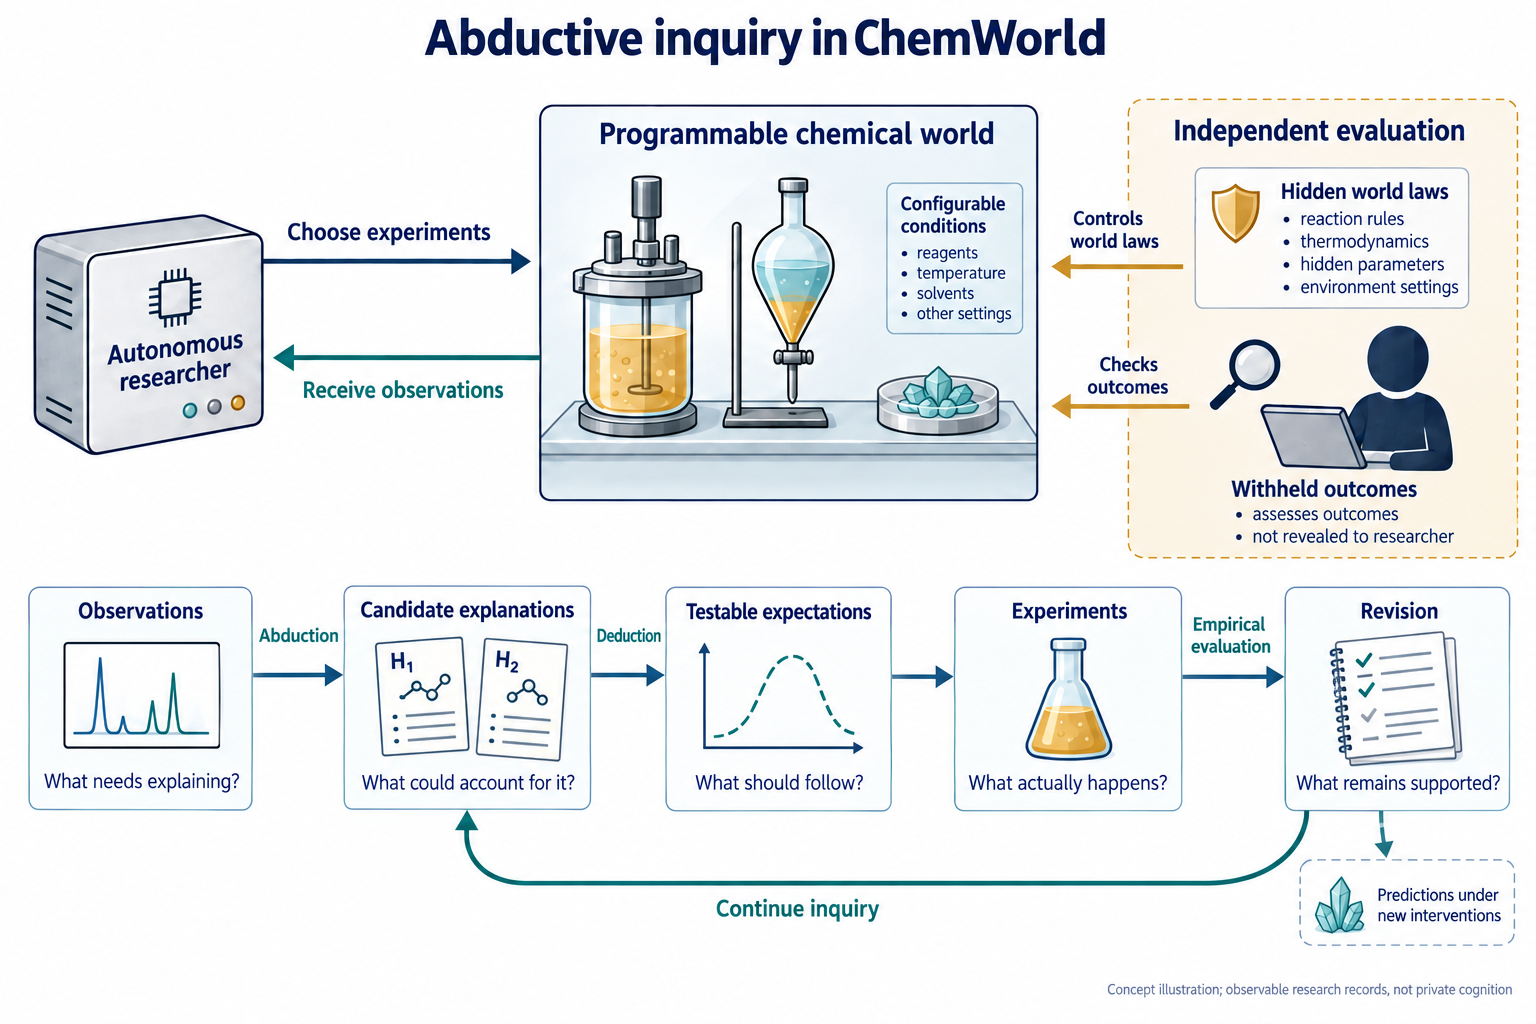
\includegraphics[width=\linewidth,height=.68\textheight,keepaspectratio]{../figures/integrated-20261016/abductive_inquiry.png}}
\caption{图 1 \textbar{} 作为可观察研究过程的反绎探索。ImageGen 概念图。自主研究者选择干预，从持续状态的化学世界获得公开观测；评估者独立控制隐藏规律并核对封存结果。下方循环区分候选解释的提出、可检验预期的推导、实验执行和支持范围的修订。修订后的判断可指导后续探索和新干预下的预测。这是分析可观察研究记录的框架，不表示每个动作均完成该循环，也不是内部认知的直接读数。}
\end{figure*}

\subsection{研究目标与先验知识组织科学探索}\label{ux7814ux7a76ux76eeux6807ux4e0eux5148ux9a8cux77e5ux8bc6ux7ec4ux7ec7ux79d1ux5b66ux63a2ux7d22}

探索始于研究目标、可用信息和受约束的行动空间。历史电化学与反应研究分别要求智能体发展并检验科学理解，或优化公开的操作评分。这些任务产生了实际实验成果，但操作和预测的收益并不可以互相替代（图 2a,b）。30 组匹配的电化学比较中，优化任务在 26 组取得更好的独立复测方案；其中十三组的预测误差更低，另十三组更高。反应处理中，发现任务在三十组中的十七组同时取得更好方案和更准确的评分预测。研究目标与科学后果之间的关系，因而需要结合探索实际建立了什么来理解。

一组电化学研究使这一区别具体可见（图 2c,d）。发现任务先比较材料与条件，再增加时长和电流上限；优化任务先筛选材料组合，再围绕有希望的组合调整操作条件。优化推荐的复测评分为 0.756，高于发现任务的 0.718，但预测平均绝对误差（MAE）为 0.229，高于 0.088。优化研究者在后续预测理由中，将若干表现不佳的交叉材料组合概括为低活性。对于其中一个组合的新条件，它预测 0.070，而参考为 0.494；另一个预测仍准确，为 0.570 对 0.572。这些经历揭示了单一终点评分无法说明的差别：成功开发实验方案，可以与对更广实验空间的不均衡判断并存。

先验信息提供了进入研究组织过程的另一切入口。修正版结晶中，Aligned 条件的十五场均从溶剂 S2、催化剂 C1 开始；没有实例资料的十五场均从 S0、C0 开始。指定错配资料下，十三场从 S2 开始，十四场首先使用 C1。Aligned、Opaque、MisIndexed 的平均实际使用溶剂数分别为 2.93、4.00、2.40。这些描述性差异显示给定信息如何进入材料选择；覆盖更广本身并不证明学习更好。反应处理中，部分参数知识具有明确的预测收益：Aligned 将发现目标的宏平均 MAE 从 0.102 降至 0.057，将优化目标的误差从 0.139 降至 0.084，在两类目标下均于五世界中的四个优于 Opaque。

\begin{figure*}[t]
\centering
\pandocbounded{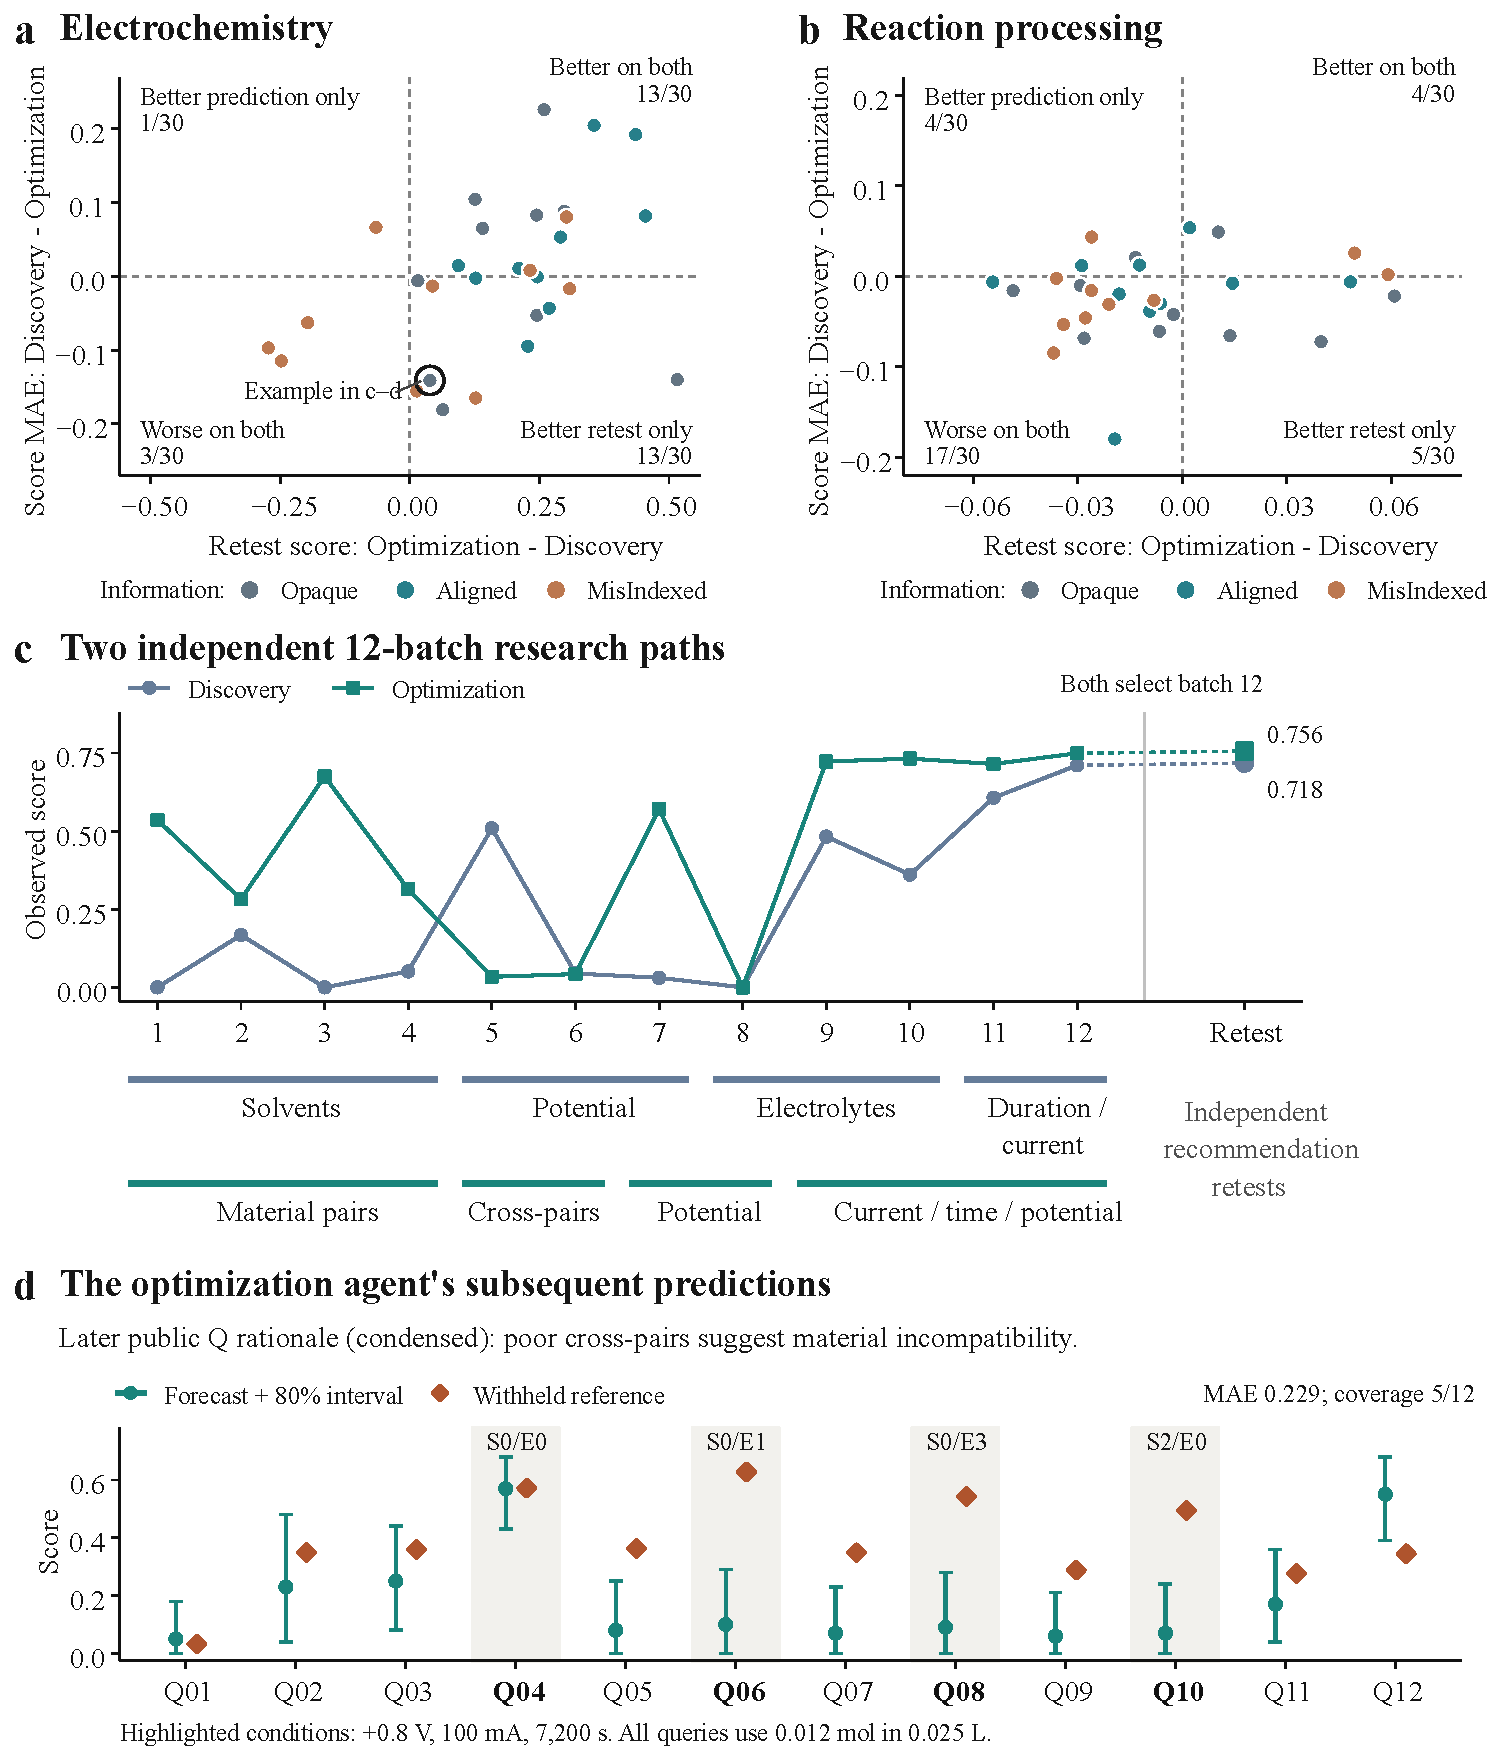
\includegraphics[width=\linewidth,height=.68\textheight,keepaspectratio]{../figures/integrated-20261016/research_objectives.pdf}}
\caption{图 2 \textbar{} 不同研究目标下的实验成果与预测理解。a、b，电化学与反应处理各三十组发现---优化匹配研究；横轴为正表示优化任务的复测评分更高，纵轴为正表示优化任务的预测 MAE 更低，象限标签均相对发现任务评价优化任务。c，两条独立的十二批电化学轨迹及推荐复测，阶段标签概括实际选择。d，该配对中优化研究者的全部十二道预测、原始 80\% 区间及封存参考；后续预测理由为压缩表述，不是同期假说记录。本图保留历史协议，不与重复过程队列合并。}
\end{figure*}

研究资源也支持不同类型的进展。历史上独立开展的十二批与二十四批研究，在一些电化学、分配和结晶预测上取得改善，却未同步增加合格结晶推荐数或平均复测回收率。这是完整资源范围的比较，不是同一研究经历的匹配继续。结合图 2 的目标比较，它们说明，更有效的操作方案或更大的实验预算，都不能单独说明研究者学到了什么科学关系。

\subsection{解释在猜想、检验与修订中发展}\label{ux89e3ux91caux5728ux731cux60f3ux68c0ux9a8cux4e0eux4feeux8ba2ux4e2dux53d1ux5c55}

同期记录使我们能够区分继续预定扫描，与回应观测而修订解释。这些活动可能覆盖相近的实验空间。例如，历史电化学发现与优化任务的溶剂覆盖接近，在较大预算下均覆盖全部四种溶剂，操作和预测结果却不同。因此，为考察解释性探索，我们追踪原先预期什么、实际观察到什么，以及研究者随后提出检验什么。

新增研究机会比较中的一条连续轨迹，下文称为``平衡研究 A''，使这一转变具体可见（图 3）。该研究采用 Opaque 信息，没有获得实例专属的档案关系。初始笔记预期弱酸趋势：浓度升高应降低 pH 和解离分数，但前六次实验的解离分数始终约为 0.064--0.079。下一版笔记撤回原趋势在已测范围内的支持，并提出一种可选组分可能比原试剂更直接决定实际酸投料。它同时明确什么结果支持这一解释：系统性的 pH 或解离响应，或沉淀阈值；平坦响应则更支持固定背景或弱耦合解释。第八至十二批实际改用该组分，响应依然接近平台。封存解释保留局部关系，同时没有认定唯一隐藏机制。这在同一研究经历中连接了初始预期、不符观测、候选解释、具有判别意义的预期和真正执行的检验。

这一序列呈现了可观察的反绎活动：偏离初始预期的结果，引出新的解释可能及与之相关的实验。持续存在的平台仍未区分所有竞争机制。因此，证据建立了一段解释性研究和一项有边界的经验发现，尚未唯一识别隐藏规律。这一区别使我们能够在实际达到的层次上评价科学进展。

修正版结晶的 58 个窗口中，52 个所选即时计划与后续实际动作匹配，6 个部分匹配。这刻画可观察窗口中的公开计划---行动联系，不是发现率或写下笔记的作用。结合连续平衡案例，这些记录使探索的适应能够被观察：实验经历可以进入修订后的预期和后续行动。这些行动究竟建立了什么，则需要考察所形成关系的内容与范围。

\begin{figure*}[t]
\centering
\pandocbounded{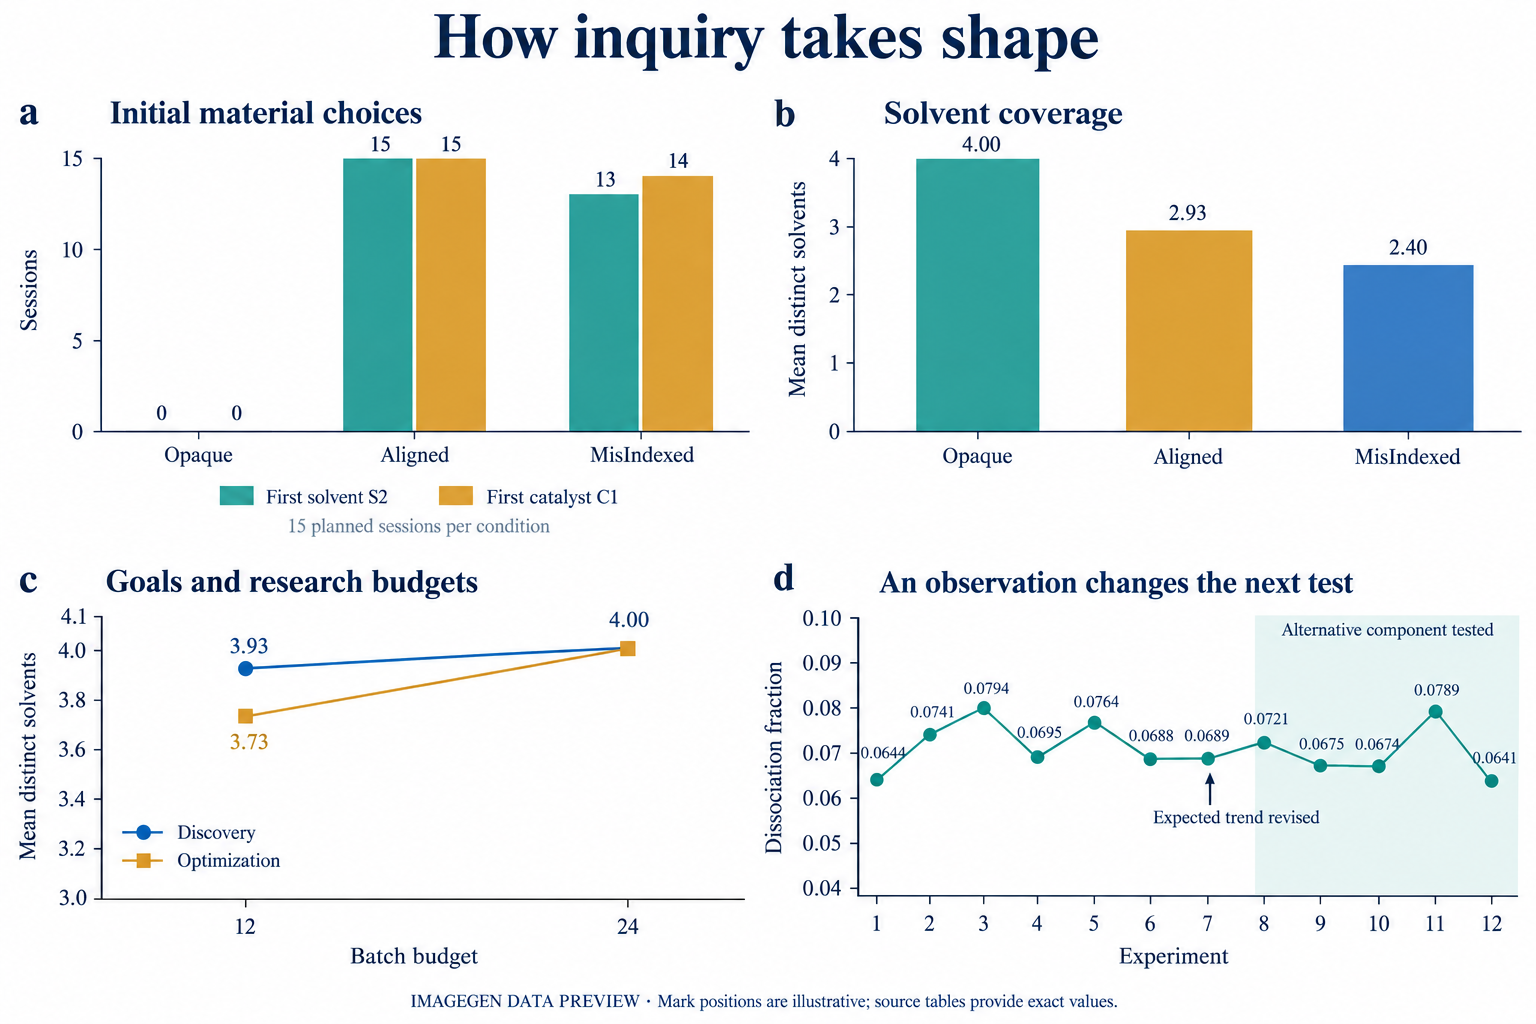
\includegraphics[width=\linewidth,height=.68\textheight,keepaspectratio]{../figures/preview-20261015/figure02.png}}
\caption{图 3 \textbar{} 平衡研究 A：从修订预期到外推。同一研究会话及其匹配无研究预测的 ImageGen 数据预览。a，前六次测定不支持初始弱酸趋势在当前范围内的适用性。b，新候选解释进入第 8--12 批替代组分检验，响应仍接近平台。c，封存解释中的局部关系随后在极稀预测中获得较大权重，引文为原文。d，研究组预测解离分数 0.085 {[}0.035, 0.350{]}，无研究组 0.569 {[}0.040, 0.980{]}，封存参考均值为 0.716。区间为研究者给出的 80\% 预测区间，源点为单次测定。这是新增研究机会比较的案例，证据包保留完整身份；生成几何为示意。}
\end{figure*}

科学关系在支持进一步检验、约束解释或指导新干预时，获得实际研究意义（图 4）。一场修正版结晶研究在获得接近细粉阈值的结果后，事前提出将试剂投料从 0.03 降至 0.02 mol。下一批执行该提议，将细粉从 0.529 降至 0.387，跨过 0.50 阈值。这支持一项局部配方改进。然而，催化剂绝对量保持不变，其相对试剂的比例也随之改变，实验未单独识别浓度机理。所建立的是被测配方与结果之间的有效关系，其支持范围窄于唯一确定的因果定律。

第二场结晶研究检验了一项插值预期。在附近溶剂体积下观察到不同回收和细粉结果后，研究者提出，0.065 L 应保留回收收益并改善细粉。下一次实验却使细粉从 0.512 增至 0.601，最终笔记撤回该预期。因此，失败的操作干预产生了明确回应证据的修订。它与低投料成功检验共同展示实验推进判断的两种方式：建立局部改进，或撤回观测不支持的预测。

一项干预是否实际发生，同样决定能够从中获得什么认识。播种案例 B 计划累计加入约 1 g 晶种，但只有 0.05 g 真正提交，随后十九次请求均被拒绝。后续笔记正确认识到，高剂量检验尚未执行。播种案例 C 遭遇类似拒绝，却将 1 g 描述为已经检验，并据此反对播种解释。这两个案例显示，对同类执行限制可以赋予不同证据意义。额外的热历史和近阈值重复案例保留在补充材料。

这些片段呈现解释性探索的不同组成部分。平衡案例包含对未预期响应的候选解释及其后果检验；结晶案例则显示事前预期、有边界的支持与修订。它们的科学价值在于，观测允许研究者保留或放弃什么。有效干预、获得支持的经验关系和已经识别的机制，是可以区分的成果，都可能进入下一次研究。

\begin{figure*}[t]
\centering
\pandocbounded{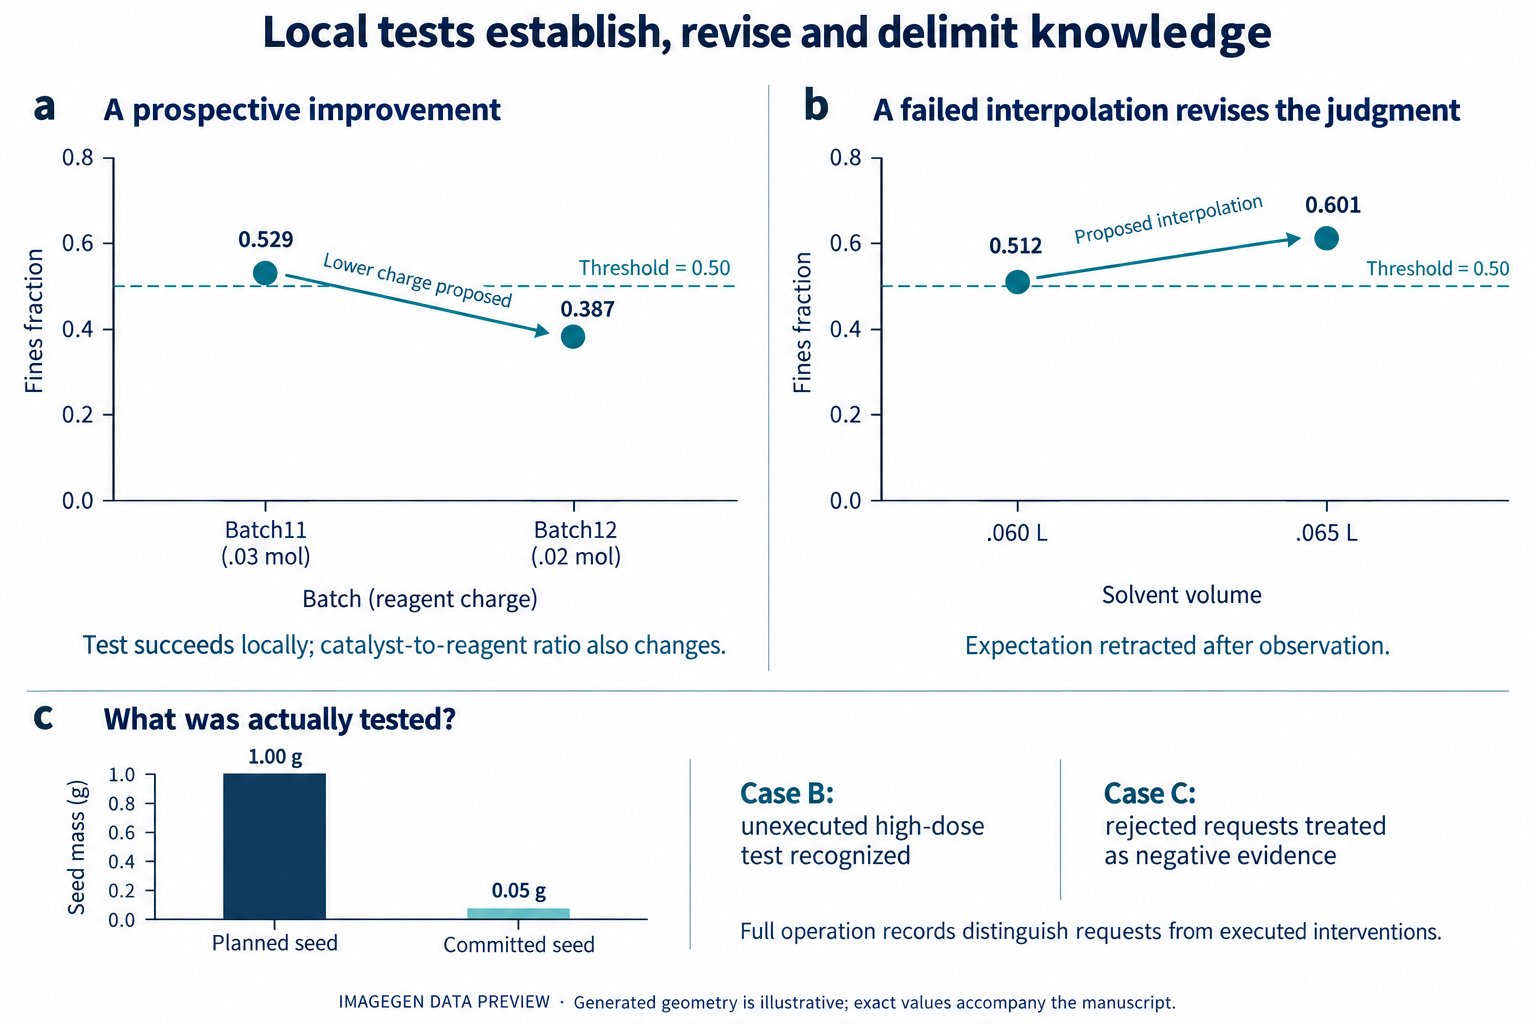
\includegraphics[width=\linewidth,height=.68\textheight,keepaspectratio]{../figures/preview-20261015/figure03.png}}
\caption{图 4 \textbar{} 局部检验建立、修订并限定认识。不同结晶研究的 ImageGen 数据预览。a，低投料使细粉从 0.529 降至 0.387，跨过 0.50 阈值，同时改变催化剂/试剂比例。b，溶剂体积插值使细粉从 0.512 增至 0.601，研究者撤回原预期。a、b 中的点是单次测定，不是带不确定性区间的均值。c，计划 1 g 的晶种添加只有 0.05 g 真正提交；案例 B 识别未执行的高剂量检验，案例 C 却将拒绝请求视为阴性证据。它们是不同研究者，不是同一轨迹的连续状态。生成几何为示意，完整记录随稿提供。}
\end{figure*}

\subsection{从局部证据走向外推的不同路径}\label{ux4eceux5c40ux90e8ux8bc1ux636eux8d70ux5411ux5916ux63a8ux7684ux4e0dux540cux8defux5f84}

相同目标与科学条件下，研究路径也会不同。五模型平衡比较允许研究者选择投料、稀释和加料顺序，再预测 pH、解离分数与沉淀。隐藏规律在较高浓度区间产生接近恒定的解离分数，在极稀条件下产生变化。Astra 的十五场研究中，十一场测量了名义浓度不高于 1 mM 的正投料样品；Sol、GPT-5.5、Luna、Terra 各十五场中均没有这样的测量（图 5a）。这一差异描述这些具体研究获得了什么证据，不定义模型固定的探索性格。

一场 Astra 研究展示了新证据的科学用途（图 5d）。前三次测定的解离分数为 6.3--7.4\%；第五批测量 18.5 微摩尔每升条件，观察到 53.8\%。后续科学解释区分高浓度平台与低浓度响应，并对 13.3 微摩尔每升条件封存预测 58.80\%，80\% 区间为 54.20--63.40\%，参考均值为 57.97\%。Sol/Opaque 则沿另一条路径获得准确预测：源研究始终未进入极稀区间，其五世界极稀宏平均 MAE 仍为 0.01833（图 5b,c）。因此，准确预测既可以伴随新响应的直接观测，也可以来自局部观测之外的外推。直接采样每个目标条件并不是成功推断的必要条件。

\begin{figure*}[t]
\centering
\pandocbounded{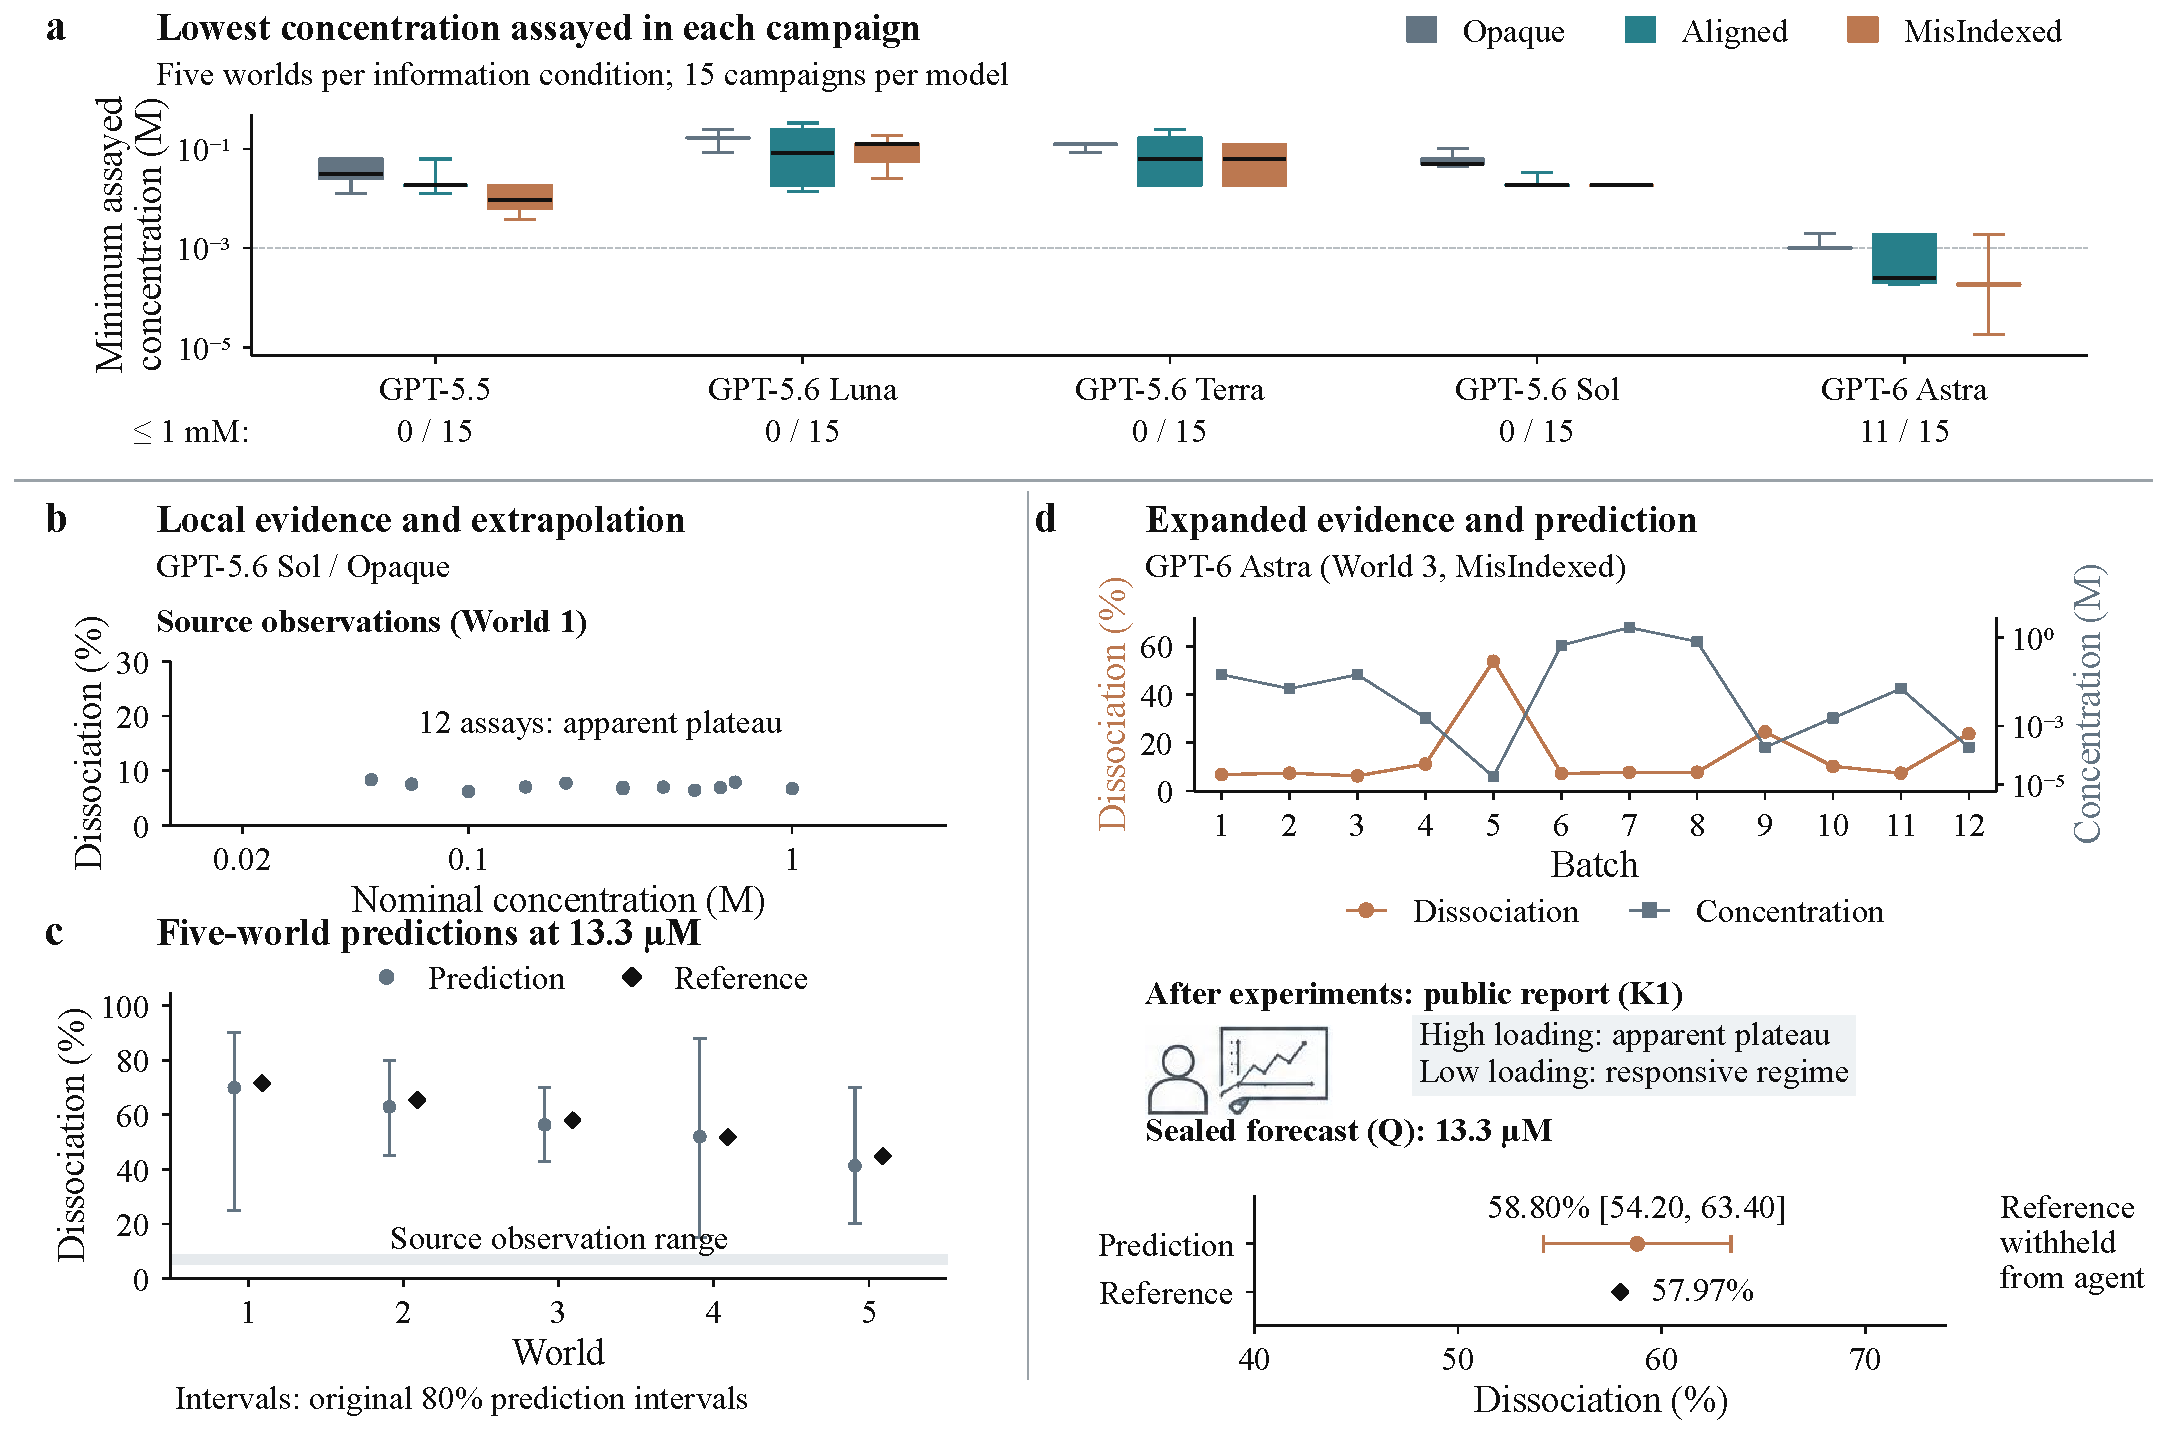
\includegraphics[width=\linewidth,height=.68\textheight,keepaspectratio]{../figures/integrated-20261016/evidence_paths.pdf}}
\caption{图 5 \textbar{} 从实验证据走向预测的不同路径。a，历史平衡 75 场研究实际测定的最低正投料浓度；每信息条件的箱体含五世界值，展示中位数、第一与第三四分位数，须为最小---最大值，四分位数在对数显示前计算，1 mM 阈值仅用于描述。b，一场 Sol/Opaque 研究的十二次源测定。c，Sol/Opaque 五世界最稀条件预测及原始 80\% 区间，阴影为源解离分数范围。d，一场 Astra/MisIndexed 的全部十二批、压缩的实验后科学解释及封存预测；解释来自事后报告，不是同期推理引文。这些数据区分扩展证据获取和局部证据之外的外推，不将任一路径认定为模型普遍的认知机制。}
\end{figure*}

关键问题在于，这些不同路径究竟建立了什么。外推可以在未直接测量每个目标条件时仍然合理，其支持程度取决于可用理论、观测与尚未解决的替代可能。沿判断的局部证据基础追踪到新的用途，使这一区别具体可见。

同一平衡研究 A 进一步连接合理的局部修订及其后续用途（图 3c,d）。预测极稀条件时，智能体写道：``The point estimate still favors the experimentally supported fixed acidic background''。它给出解离分数 0.085、80\% 区间 0.035--0.350，而封存参考均值为 0.716。科学解释与预测都承认该区间未经测试，因此问题比漏写适用范围更具体：局部受支持的关系，在实验尚未确定其延续性的预测中获得较大权重。同一道题的匹配无研究预测为 0.569，区间 0.040--0.980，明确依赖未经检验的先验假设。它在数值上更准确，并不证明其取得了更好的实验发现。

这种延续并非必然。另一个固定平衡世界中的两场研究均在较高投料下观察到平台，极稀宏平均误差却分别为 0.16287 和 0.01462。对于同一道极稀题，它们预测解离分数 0.130 和 0.626，参考均值为 0.65463。较准确的研究采用与平台观测相容的弱酸延续，并明确将其描述为猜想。结合历史 Sol/Opaque 和 Astra 案例，这些记录区分了通向判断的不同路径：观察到的变化、合理外推，以及被带入未决区域的局部关系。数值正确与通过实验确立，仍是不同问题。

平衡体系的先验比较与反应体系的正向结果形成对照。原 Sol 研究中，正确的部分信息将九道题的宏平均 MAE 从 0.01008 降至 0.00465，却将三道最稀题的误差从 0.01833 提高到 0.15862，两个方向在五个世界中均出现。另一个重复队列显示相同的总体方向、不同的幅度：九道题从 0.00907 降至 0.00512，极稀子集从 0.09880 增至 0.13205。两队列分别报告。模型比较进一步限定这一解释（图 6c）：Luna 与 Terra 在两个区域均从 Aligned 获益，GPT-5.5 变化很小，Astra 在三个信息条件下均保持较低极稀误差。部分知识的作用因而同时取决于研究者和被判断的条件；局部收益不能决定它在其他区域的价值。

\begin{figure*}[t]
\centering
\pandocbounded{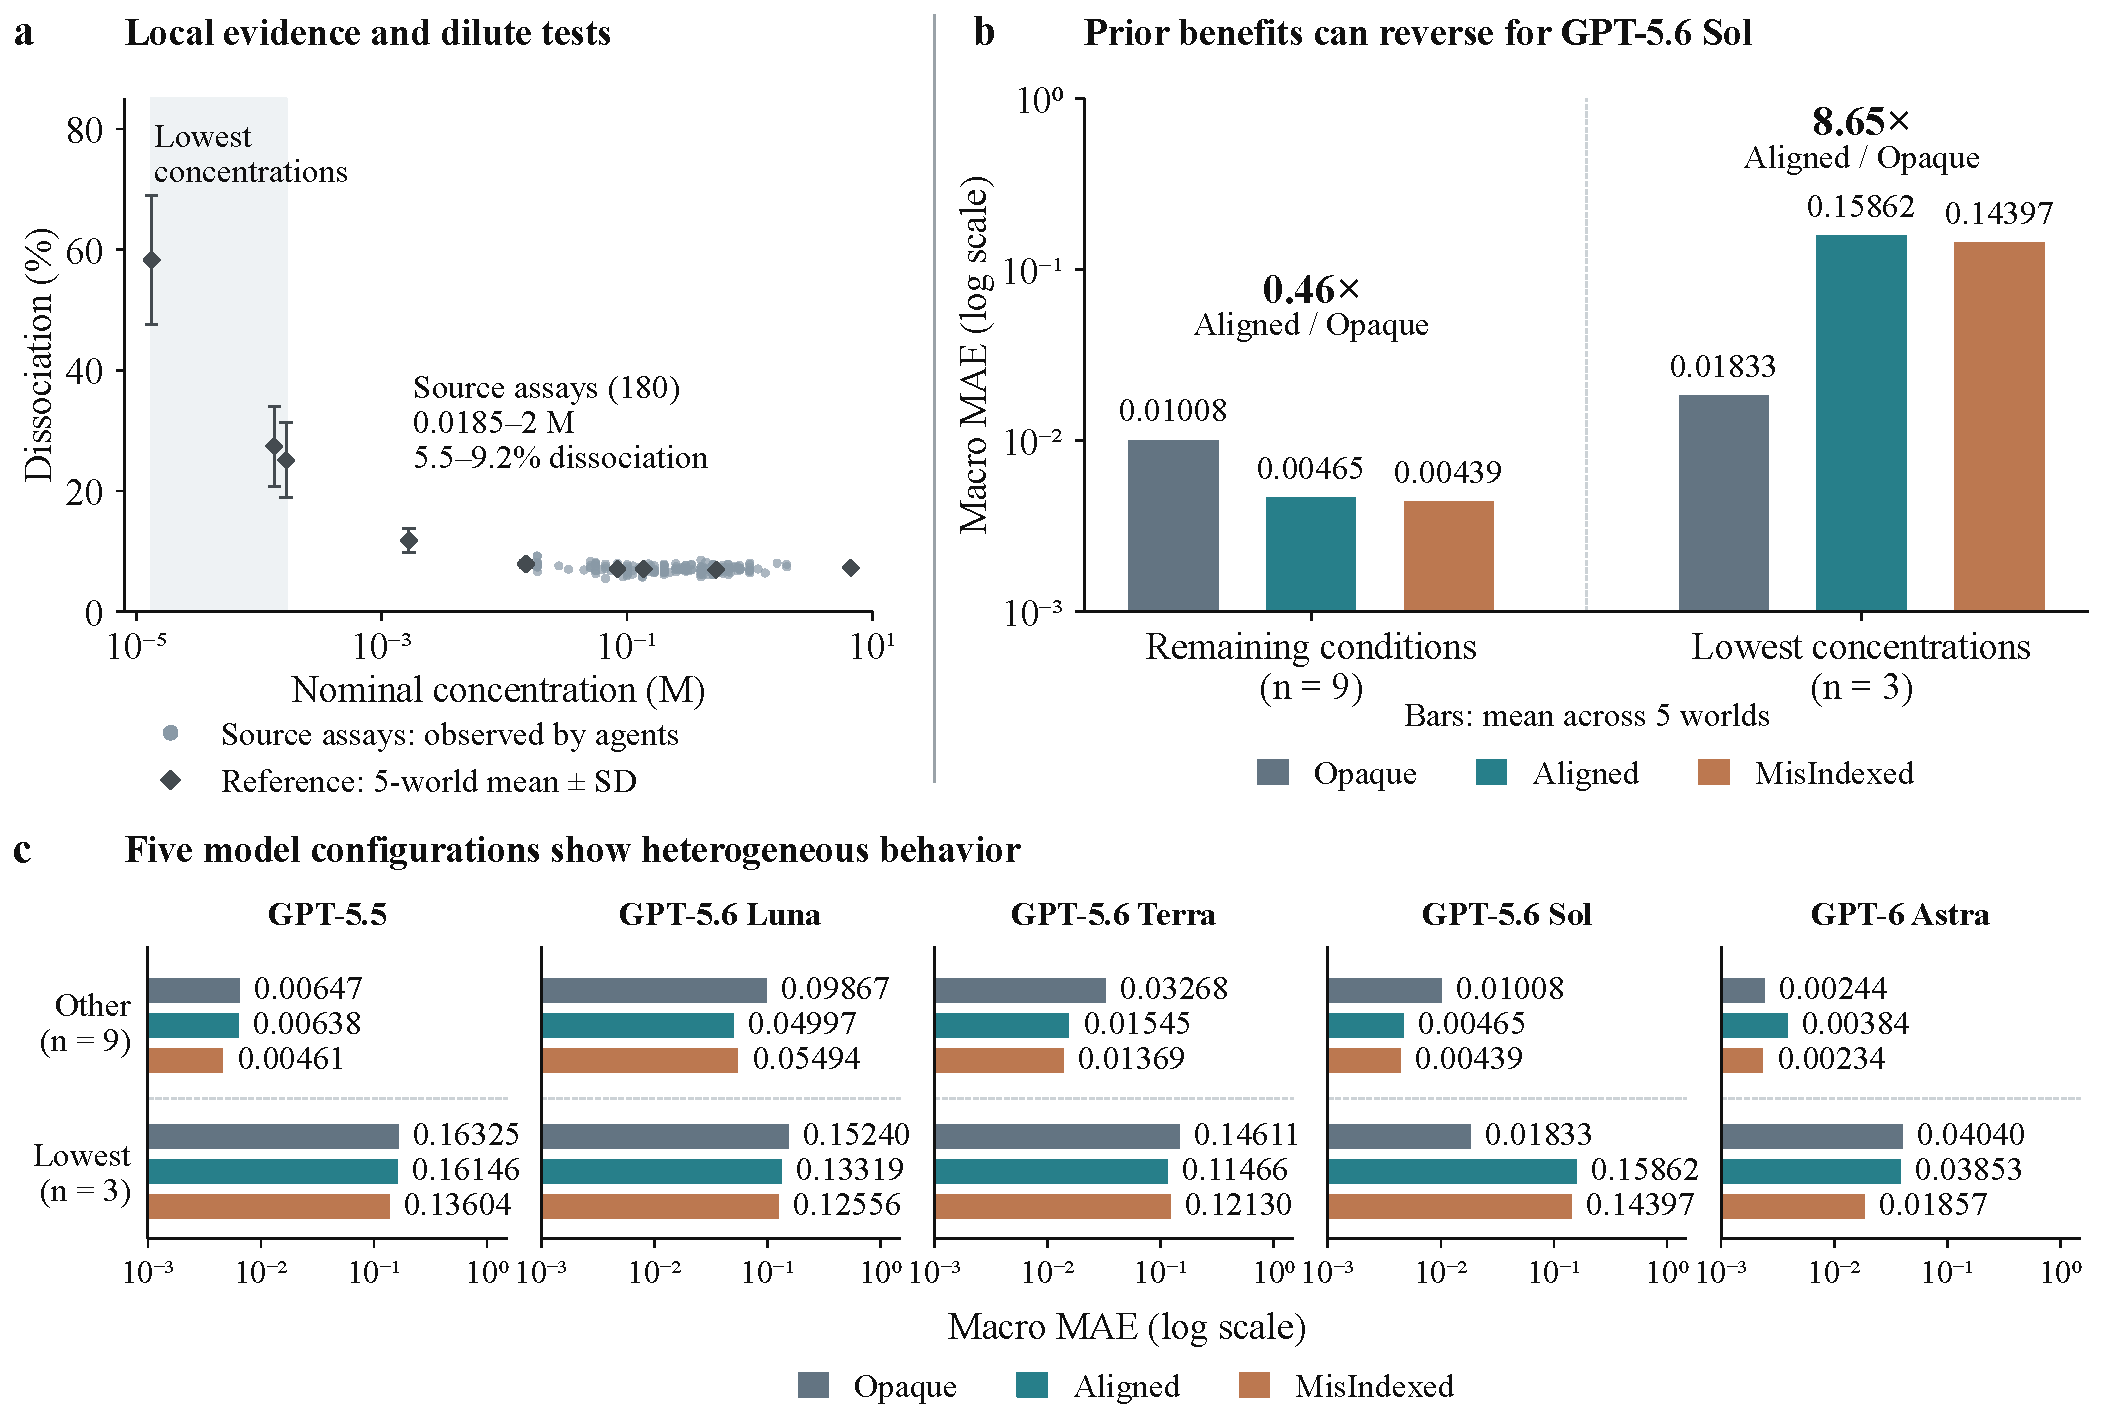
\includegraphics[width=\linewidth,height=.68\textheight,keepaspectratio]{../figures/integrated-20261016/priors_and_transfer.pdf}}
\caption{图 6 \textbar{} 部分先验知识的适用范围取决于研究者与判断条件。原平衡比较。a，Sol 的全部 180 次源测定与五世界封存题目均值，误差线为描述性样本标准差，不是置信区间。b，Sol 三种信息条件的五世界宏平均 MAE。c，五种模型配置，采用相同对数误差轴，条形基线为 0.001。最稀三题与其余九题的分组是历史队列的事后分析，在后续重复块之前固定。图中均为历史结果，正文另报的重复队列不加入这些条形。每个模型---世界---信息组合只有一次研究。}
\end{figure*}

\subsection{研究改变科学认识的适用范围}\label{ux7814ux7a76ux6539ux53d8ux79d1ux5b66ux8ba4ux8bc6ux7684ux9002ux7528ux8303ux56f4}

随着研究走出解释形成时的条件，其科学作用仍需在新的判断中体现。因此，我们以受控研究机会比较补充已经观察到的推断路径，再按响应考察已获证据如何进入新预测。

匹配的研究机会比较提出更直接的问题：在共同的初始科学信息下，获得研究机会是否改变后续预测（图 7）？三十场均采用 Opaque 信息：公开任务、材料身份、测量尺度、合法操作和初始状态可用，但不提供实例专属档案规律或拟合关系。五个平衡世界各安排三场拥有十二个源批次的新会话，以及三场不开展源实验的新会话。每世界、每重复的科学输入和封存评估相匹配。三十场全部终止，180 个计划源批次全部完成，二十九场提供有效预测。一场研究会话因网络中断缺失预测及后续阶段，其观测和科学解释仍保留。

\begin{figure*}[t]
\centering
\pandocbounded{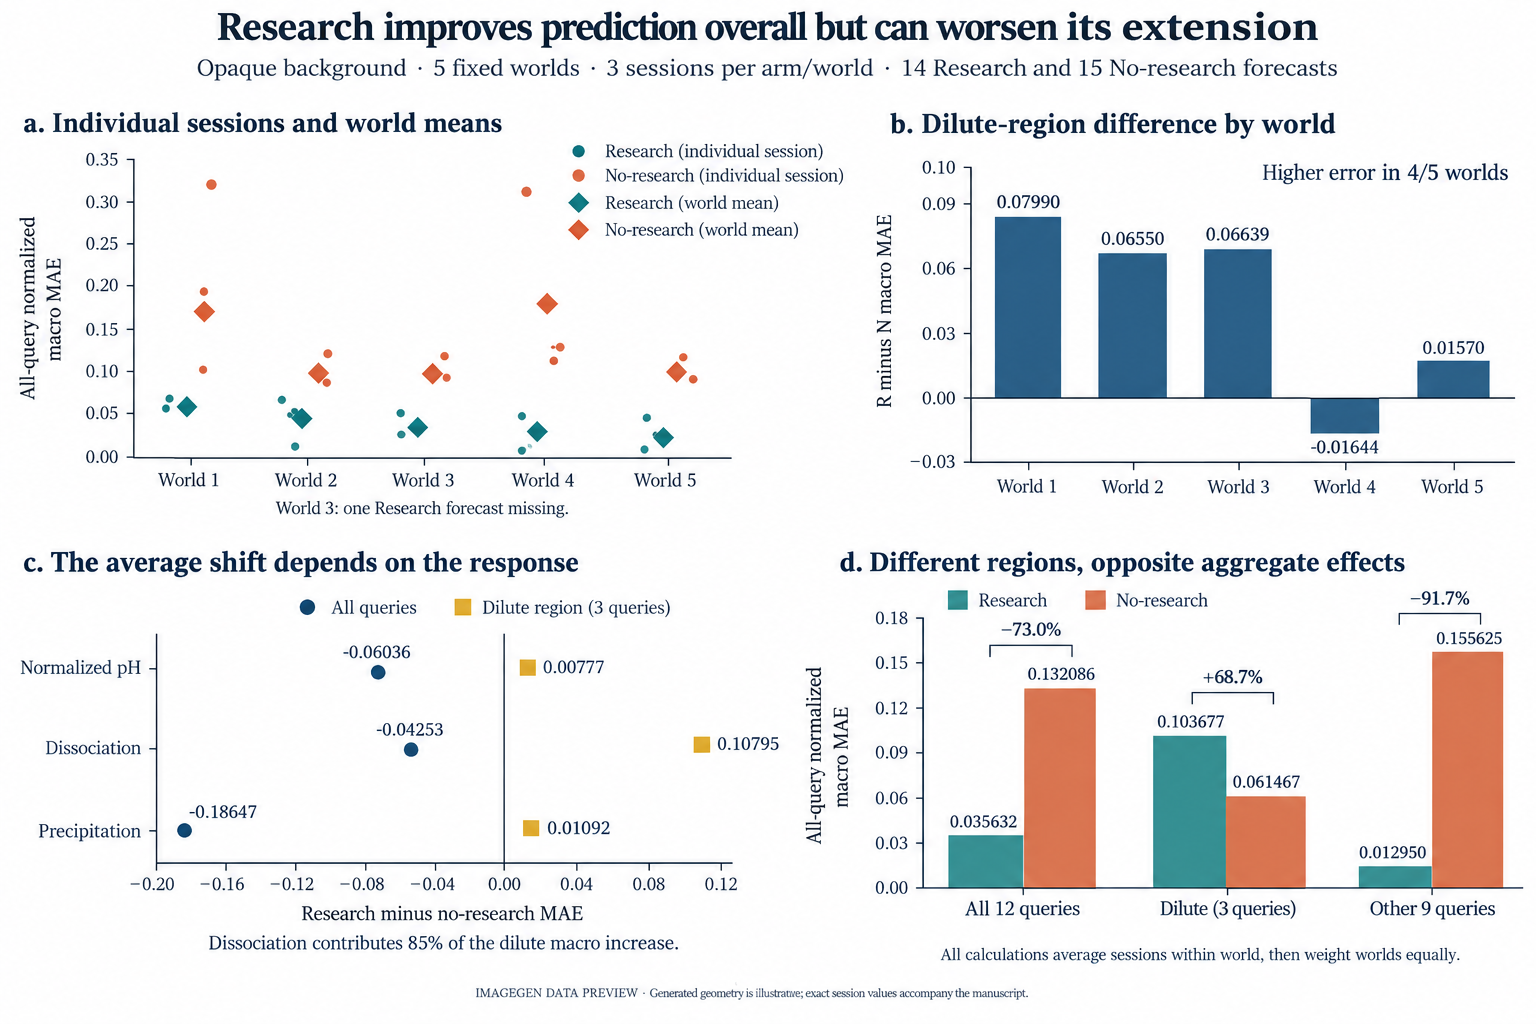
\includegraphics[width=\linewidth,height=.68\textheight,keepaspectratio]{../figures/preview-20261015/figure04.png}}
\caption{图 7 \textbar{} 研究带来的总体收益与区域反转。ImageGen 数据预览。三十场均采用 Opaque 和匹配科学输入。a，逐会话全题宏平均误差及世界内均值；研究组十四份有效预测，无研究组十五份；世界三缺失的一份研究预测保留。b，极稀区域研究减无研究的宏平均误差，在五世界中的四个为正。c，响应贡献不同，解离分数占极稀宏平均误差增量的 85.2\%。d，全部十二题、极稀三题、其余九题的等权误差分别变化 −73.0\%、+68.7\%、−91.7\%。生成点与几何为示意；准确会话值、响应误差和全部 1,044 条有效逐题逐响应记录见证据包。不表示置信区间或总体抽样推断。}
\end{figure*}

研究总体上大幅降低了预测误差。先在每世界内平均有效会话，再对五世界等权，归一化宏平均绝对误差由无研究的 0.132086 降至研究的 0.035632，降低 73.0\%，五个世界方向一致。然而，在三道事前指定的极稀题上，误差由 0.061467 增至 0.103677，提高 68.7\%，五世界中四个恶化；其余九道题从 0.155625 降至 0.012950。比较针对完整研究机会，包括实验选择、反馈和可用记录工具，不分离其中任一成分。

在这一比较中，同一研究机会改善了总体预测，却使特定区域的预测变差。极稀子集中三项响应的平均点误差均增加，幅度不同：研究减无研究的 MAE 分别为归一化 pH +0.00777、解离分数 +0.10795、沉淀信号 +0.01092。解离分数占宏平均误差增量的 85.2\%。图 7 展示逐会话与世界均值，完整逐会话、逐响应、逐题结果随稿提供。平衡研究 A 提供从有效局部发现走向远端判断的一条可见路径，不证明它解释每场差异，也不意味着获得更多证据必然损害外推。

这一结果也体现在区间评价中，但不支持普遍的错误自信故事。极稀条件下，研究组的三项名义 80\% 区间均有更低的经验覆盖率，无研究区间则宽得多。同时惩罚宽度和遗漏的区间分数，对 pH 更有利于研究，对解离分数更有利于无研究，对沉淀信号相近。在全部题目上，研究均改善三项区间分数。允许缺失会话的宏平均误差取合法范围内任何值的保守敏感性分析，不改变总体获益与极稀恶化两个方向（方法）。

结晶呈现了已获证据使用中的互补情形（扩展数据图 2）。对 42 份有效预测，透明参照仅使用该会话自己的源观测。五世界等权纯度误差，智能体为 0.03853、源均值为 0.00510，后者在每场有效研究中都更准确；回收表现相反，智能体误差为 0.10129，源均值为 0.20443，智能体在 39/42 场获胜。按实际提交的溶剂集合匹配，两个总体方向仍保留。粒径与细粉分别为 5/42、23/42 场优于源均值。这些参照诊断不同响应中对已获证据的使用，不是无研究对照或另一个自主研究者，也不估计结晶研究的因果收益。

这一响应差异补充了平衡结果。挑战不仅在于预见已观察区域之外的变化，也在于保留仍然有效的关系。同一结晶经历中，预测比源均值更有效地利用了变化的回收信息，却未能在稳定纯度上达到这一简单参照。一个响应中的成功证据使用，不证明所有已获关系都同等约束后续判断。贯穿目标、先验、预算和研究机会，科学进展因此具有多个可观察维度：实验取得什么成果，证据确立什么关系，以及这些关系怎样指导新判断。

\FloatBarrier
\subsection{讨论}\label{ux8ba8ux8bba}

反绎探索为自主科学提供了具有实质内容的评价对象：解释如何通过研究得到发展。本文连接智能体开展探索的条件、公开提出的假说与关系、实际执行的检验，以及随后形成的判断。跨体系比较显示，操作成功与预测理解可以沿不同方向发展；同期案例则说明，这种分化可以与有意义的科学活动并存，包括提出替代解释、检验局部预期，以及在观测不符时将其撤回。分析的单位是置于研究经历中的解释，以及赋予其科学意义的证据与用途。

结果区分了解释的提出、实验证据支持和成功应用。在平衡研究 A 中，合理的候选解释引出实际检验，却未唯一确定隐藏机制；结晶中，成功的配方变化建立有效干预，同时留下相关原因未决，失败的插值则支持合理撤回。Astra 与 Sol/Opaque 的经历进一步显示，准确预测可以来自对响应变化的直接观察，也可以来自局部证据之外的猜想性延续。这些是不同的科学成果。若将所有实验视为可以互换的数据采集，或将所有正确预测视为等价的发现证据，就会失去这些区别。

这一视角将反绎放回与演绎及经验检验的持续交互中。候选解释为观测提供一种可能说明，其推论指导检验，结果又可以增强、限定或取代该解释。实证记录也呈现这种联系在哪里没有充分建立：被拒绝的操作可能被记为已完成检验，局部规律可能主导尚未解决的外推，已经建立的响应也可能未约束预测。因此，发现与误解可以出现在同一探索的不同环节。考察这些转变，使我们能够同时追问结论是否正确，以及研究者有何理由得出这一结论\textsuperscript{12,22,23}。

受控比较为这一过程解释提供补充。研究目标、先验信息与可用资源揭示探索的不同条件；匹配机会研究则在共同初始信息下，考察开展研究的总体贡献。其中的总体收益与区域反转说明，科学收益可以随所问问题变化，却不分离反绎、自主性、反馈或笔记的独立作用。固定配方淬灭比较识别干预的物理后果，并未向可适应的智能体反馈结果（扩展数据图 3）。公开判断与行动的时间联系，同样不确立判断形成的唯一因果机制。这些区别使不同比较能够贡献于同一问题，同时保留各自的因果解释范围。

研究限于选定的可编程系统和少数固定世界，重复过程分析采用一种模型配置。新会话不是受控模型 seed 重复，也不是世界规律的独立抽样。公开笔记不揭示内部认知，可观察的解释性活动也不等于发明新的科学理论。该框架组织对已有证据的解释，未新增反绎能力的定量测试。案例事后选择，由单一分析者解释，没有第二编码者一致性估计。历史与当前协议保留各自来源，包括修正版结晶及全部失败。这些边界界定了当前证据支持解释形成、检验与使用的尺度。

更广的研究雄心，是理解一个能够开展实验的系统，如何成为能够发展科学解释的系统。爱因斯坦的例子提出这一智力要求，可编程世界则使其中的具体环节进入受控研究范围。ChemWorld 将智能体提出的解释、据此选择的实验，以及能够改变其世界认识的证据联系起来。科学自主性在这种持续回应中发展：能够追究一种解释，确定它究竟建立了什么，并随探索推进而修订其适用范围。

\subsection{资助}\label{ux8d44ux52a9}

本研究获得深圳市科技计划项目（AI2026004）、清华大学自主科研计划，以及青年教师科研创新能力支持项目（ZYGXQNJSKYCXNLZCXM-E7）资助。

\clearpage
\onecolumn

\section{参考文献}\label{ux53c2ux8003ux6587ux732e}

\protect\phantomsection\label{refs}
\begin{CSLReferences}{0}{1}
\hypertarget{ref-einstein1905electrodynamics}{}
\CSLLeftMargin{1. }%
\CSLRightInline{A. Einstein. Zur elektrodynamik bewegter k{ö}rper. \emph{Annalen der Physik} \textbf{322} 891--921 (1905). https://doi.org/\href{https://doi.org/10.1002/andp.19053221004}{10.1002/andp.19053221004}.}

\hypertarget{ref-douven2025peirce}{}
\CSLLeftMargin{2. }%
\CSLRightInline{I. Douven. Peirce on abduction. \emph{The stanford encyclopedia of philosophy: abduction} (2025). \url{https://plato.stanford.edu/entries/abduction/peirce.html}.}

\hypertarget{ref-tom2024selfdriving}{}
\CSLLeftMargin{3. }%
\CSLRightInline{G. Tom et al. {Self-Driving Laboratories for Chemistry and Materials Science}. \emph{Chemical Reviews} \textbf{124} 9633--9732 (2024). https://doi.org/\href{https://doi.org/10.1021/acs.chemrev.4c00055}{10.1021/acs.chemrev.4c00055}.}

\hypertarget{ref-boiko2023autonomous}{}
\CSLLeftMargin{4. }%
\CSLRightInline{D. A. Boiko, R. MacKnight, B. Kline, and G. Gomes. Autonomous chemical research with large language models. \emph{Nature} \textbf{624} 570--578 (2023). https://doi.org/\href{https://doi.org/10.1038/s41586-023-06792-0}{10.1038/s41586-023-06792-0}.}

\hypertarget{ref-king2009automation}{}
\CSLLeftMargin{5. }%
\CSLRightInline{R. D. King et al. {The Automation of Science}. \emph{Science} \textbf{324} 85--89 (2009). https://doi.org/\href{https://doi.org/10.1126/science.1165620}{10.1126/science.1165620}.}

\hypertarget{ref-burger2020mobile}{}
\CSLLeftMargin{6. }%
\CSLRightInline{B. Burger et al. {A mobile robotic chemist}. \emph{Nature} \textbf{583} 237--241 (2020). https://doi.org/\href{https://doi.org/10.1038/s41586-020-2442-2}{10.1038/s41586-020-2442-2}.}

\hypertarget{ref-macleod2020selfdriving}{}
\CSLLeftMargin{7. }%
\CSLRightInline{B. P. MacLeod et al. {Self-driving laboratory for accelerated discovery of thin-film materials}. \emph{Science Advances} \textbf{6} eaaz8867 (2020). https://doi.org/\href{https://doi.org/10.1126/sciadv.aaz8867}{10.1126/sciadv.aaz8867}.}

\hypertarget{ref-szymanski2023alab}{}
\CSLLeftMargin{8. }%
\CSLRightInline{{N. J. Szymanski et al.} An autonomous laboratory for the accelerated synthesis of inorganic materials. \emph{Nature} \textbf{624} 86--91 (2023). https://doi.org/\href{https://doi.org/10.1038/s41586-023-06734-w}{10.1038/s41586-023-06734-w}.}

\hypertarget{ref-bran2024augmenting}{}
\CSLLeftMargin{9. }%
\CSLRightInline{A. M. Bran et al. Augmenting large language models with chemistry tools. \emph{Nature Machine Intelligence} \textbf{6} 525--535 (2024). https://doi.org/\href{https://doi.org/10.1038/s42256-024-00832-8}{10.1038/s42256-024-00832-8}.}

\hypertarget{ref-dai2024mobile}{}
\CSLLeftMargin{10. }%
\CSLRightInline{T. Dai et al. {Autonomous mobile robots for exploratory synthetic chemistry}. \emph{Nature} \textbf{635} 890--897 (2024). https://doi.org/\href{https://doi.org/10.1038/s41586-024-08173-7}{10.1038/s41586-024-08173-7}.}

\hypertarget{ref-elmachtoub2022spo}{}
\CSLLeftMargin{11. }%
\CSLRightInline{A. N. Elmachtoub and P. Grigas. Smart {Predict, then Optimize}. \emph{Management Science} \textbf{68} 9--26 (2022). https://doi.org/\href{https://doi.org/10.1287/mnsc.2020.3922}{10.1287/mnsc.2020.3922}.}

\hypertarget{ref-shmueli2010explain}{}
\CSLLeftMargin{12. }%
\CSLRightInline{G. Shmueli. {To Explain or to Predict?} \emph{Statistical Science} \textbf{25} 289--310 (2010). https://doi.org/\href{https://doi.org/10.1214/10-sts330}{10.1214/10-sts330}.}

\hypertarget{ref-platt1964inference}{}
\CSLLeftMargin{13. }%
\CSLRightInline{J. R. Platt. {Strong Inference}. \emph{Science} \textbf{146} 347--353 (1964). https://doi.org/\href{https://doi.org/10.1126/science.146.3642.347}{10.1126/science.146.3642.347}.}

\hypertarget{ref-lindley1956information}{}
\CSLLeftMargin{14. }%
\CSLRightInline{D. V. Lindley. {On a Measure of the Information Provided by an Experiment}. \emph{The Annals of Mathematical Statistics} \textbf{27} 986--1005 (1956). https://doi.org/\href{https://doi.org/10.1214/aoms/1177728069}{10.1214/aoms/1177728069}.}

\hypertarget{ref-chaloner1995design}{}
\CSLLeftMargin{15. }%
\CSLRightInline{K. Chaloner and I. Verdinelli. {Bayesian Experimental Design: A Review}. \emph{Statistical Science} \textbf{10} 273--304 (1995). https://doi.org/\href{https://doi.org/10.1214/ss/1177009939}{10.1214/ss/1177009939}.}

\hypertarget{ref-mirza2025chembench}{}
\CSLLeftMargin{16. }%
\CSLRightInline{A. Mirza et al. {A framework for evaluating the chemical knowledge and reasoning abilities of large language models against the expertise of chemists}. \emph{Nature Chemistry} \textbf{17} 1027--1034 (2025). https://doi.org/\href{https://doi.org/10.1038/s41557-025-01815-x}{10.1038/s41557-025-01815-x}.}

\hypertarget{ref-majumder2025discoverybench}{}
\CSLLeftMargin{17. }%
\CSLRightInline{B. P. Majumder et al. {DiscoveryBench: Towards Data-Driven Discovery with Large Language Models}. \emph{{International Conference on Learning Representations}} \textbf{2025} 4556--4579 (2025). \url{https://proceedings.iclr.cc/paper_files/paper/2025/file/0d70af566e69f1dfb687791ecf955e28-Paper-Conference.pdf}.}

\hypertarget{ref-wang2022scienceworld}{}
\CSLLeftMargin{18. }%
\CSLRightInline{R. Wang, P. Jansen, M.-A. Côté, and P. Ammanabrolu. {ScienceWorld: Is your Agent Smarter than a 5th Grader?} \emph{Proceedings of the 2022 conference on empirical methods in natural language processing} 11279--11298 (2022). https://doi.org/\href{https://doi.org/10.18653/v1/2022.emnlp-main.775}{10.18653/v1/2022.emnlp-main.775}.}

\hypertarget{ref-jansen2024discoveryworld}{}
\CSLLeftMargin{19. }%
\CSLRightInline{P. Jansen et al. {DiscoveryWorld}: A virtual environment for developing and evaluating automated scientific discovery agents. \emph{Advances in neural information processing systems} \textbf{37} (2024). https://doi.org/\href{https://doi.org/10.52202/079017-0324}{10.52202/079017-0324}.}

\hypertarget{ref-gandhi2025boxinggym}{}
\CSLLeftMargin{20. }%
\CSLRightInline{K. Gandhi et al. {BoxingGym}: Benchmarking progress in automated experimental design and model discovery. (2025). \url{https://arxiv.org/abs/2501.01540}.}

\hypertarget{ref-chen2025physgym}{}
\CSLLeftMargin{21. }%
\CSLRightInline{Y. Chen, P. Piękos, M. Ostaszewski, F. Laakom, and J. Schmidhuber. {PhysGym: Benchmarking LLMs in Interactive Physics Discovery with Controlled Priors}. \emph{{Advances in Neural Information Processing Systems}} \textbf{38} (2025). https://doi.org/\href{https://doi.org/10.52202/085713-1556}{10.52202/085713-1556}.}

\hypertarget{ref-gneiting2007scoring}{}
\CSLLeftMargin{22. }%
\CSLRightInline{T. Gneiting and A. E. Raftery. {Strictly Proper Scoring Rules, Prediction, and Estimation}. \emph{Journal of the American Statistical Association} \textbf{102} 359--378 (2007). https://doi.org/\href{https://doi.org/10.1198/016214506000001437}{10.1198/016214506000001437}.}

\hypertarget{ref-ovadia2019uncertainty}{}
\CSLLeftMargin{23. }%
\CSLRightInline{Y. Ovadia et al. {Can you trust your model's uncertainty? Evaluating predictive uncertainty under dataset shift}. \emph{{Advances in Neural Information Processing Systems}} \textbf{32} (2019). \url{https://proceedings.neurips.cc/paper_files/paper/2019/file/8558cb408c1d76621371888657d2eb1d-Paper.pdf}.}

\end{CSLReferences}

\clearpage

\section{方法}\label{ux65b9ux6cd5}

\subsection{世界、接口与实验单位}\label{ux4e16ux754cux63a5ux53e3ux4e0eux5b9eux9a8cux5355ux4f4d}

ChemWorld 将兼容的过程组件编译为具有持续状态的虚拟化学环境。公开契约指定材料、合法操作、仪器、资源和任务目标，私有参数决定具体世界的响应。智能体能够访问实验室和公开记录，不能访问评估者状态、模拟器代码、私有参数或封存参考结果。操作改变样品，测量可能消耗材料。候选转变在提交之前接受校验；被拒绝的操作不构成所请求的物理干预，但尝试可能消耗契约规定的资源。精确重放核对环境状态转变，不重新生成模型决策。

广度研究覆盖电化学、分配、反应与热处理、水溶液平衡、反应耦合结晶和纯化。这些是受控虚拟系统，不是对具名现实物质经过实验验证的预测。当前重复研究采用平衡与结晶。五个固定世界在不同条件与重复中复用，世界参数、初始状态和键控观测映射保持固定。重复单位是新模型会话，不是独立世界抽样或受控模型 seed 重复。接口没有可用的模型采样 seed；相同干预可以得到相同键控观测，因此也不是独立噪声实现。

\subsection{证据层与保留分母}\label{ux8bc1ux636eux5c42ux4e0eux4fddux7559ux5206ux6bcd}

历史广度研究包含 240 场 Sol-medium 研究，以及 Luna、Terra、GPT-5.5 和 Astra 的 60 场额外平衡研究，均请求 medium 推理强度。五模型平衡比较中的十五场 Sol 已包含在 240 场内。请求的模型标签不代表实际计算量相等。原 240 场包含电化学 60、分配 30、反应 60、平衡 45、结晶 30 和纯化 15 场；按其原规则保留 3,597/3,600 次最终测量、全部 720 个后测阶段与 238 场协议符合研究。额外六十场保留 720 批和 240 个阶段。两场原始源研究完成度失败仍予保留。更早的选定笔记案例另有 24 场，不与广度或当前过程队列合并。

当前过程队列由早期 48 场及其 42 场扩展中的 45 场平衡研究，以及统一回收描述后完整重跑的 45 场结晶研究组成。每个体系覆盖五世界、Opaque/Aligned/MisIndexed 三信息条件、每格三场，每场十二批。平衡保留 39 条完整链、41 份有效预测；修正版结晶分别为 41 和 42。当前合计分母为 90 场、80 条完整链、83 份有效预测。旧结晶作为受协议影响的历史证据保留，不加入修正版计算当前结果或过程频率。

修正版结晶完成 510/540 个源批次、125/135 个后测阶段，保留 145 版笔记和 42 次推荐复测。全部 45 条源轨迹与 42 条复测轨迹通过重放。四条不完整链中，三条缺失预测，另一条有有效预测但缺失随后的反思。平衡子集与独立的研究机会块各自保留失败表。缺失不填零，已完成结果不由后来更有利的结果替代。稿件整合不改变任何实验块原有的开发或资格证据地位。

\subsection{信息、自主性与记录}\label{ux4fe1ux606fux81eaux4e3bux6027ux4e0eux8bb0ux5f55}

历史目标比较在世界、信息条件、批次预算和先验位置内，匹配独立开展的发现与优化研究。电化学的十二与二十四批条件合计三十对；反应处理的参数和结构先验块均采用十二批，合计三十对。操作结果来自封存推荐的独立复测。联合结果计数采用公开评分的预测 MAE，反应先验比较则采用六项归一化响应误差的平均值，两者不互换。预算比较同样涉及具有完整资源范围的独立会话，不估计继续同一项研究的作用。

历史五模型平衡比较包含五世界、三信息条件，每格一场十二批研究，共七十五场，其中十五场 Sol 已计入广度研究。1 mM 阈值描述实际测量的最低正投料名义浓度，不是发现判据。浓度按名义配方投料计算，三道极稀评估题在模型配置间相同。各条件的预测误差、原始预测区间与已获证据均保留。选定的 Astra 和电化学轨迹属于事后过程示例，其科学解释在实验后写成，不是同期笔记记录，也不是额外重复。完整历史设计、响应表和案例数值保留在补充材料。

Opaque 提供公开任务和操作背景，不提供额外实例资料。Aligned 提供与体系相符的部分信息；平衡包括有效酸度区间和带锚点的局部稀释关系。MisIndexed 使用另一世界的历史关系，格式与限定相同。结晶 Aligned 提供匿名材料名义描述，MisIndexed 交换 S1/S3 溶剂描述，保留 S0、S2 和催化剂描述。两者均不是完整世界规律。

原平衡 Opaque/Aligned 早于 MisIndexed 扩展；修正版结晶是更晚的完整实验块。这些描述性比较并非全部同期随机处理，新旧结晶也不能估计修正提示的因果作用。下文单列的新研究机会比较采用共同的同期协议。

智能体在固定预算内选择操作、用量、测量、重复与操作分组。平衡允许十二批、180 次操作尝试、十二次中间仪器与十二次最终测量；结晶采用固定十二批材料预算和 720 次尝试上限。记录角色要求在适用时先写出可检验预期，后续由智能体自主更新，不要求每批书写，也不自动重新注入笔记。记录角色可能影响研究，不被视为被动观察。笔记保存版本与公开事件游标，不揭示内部认知。没有调用笔记读取工具，不代表无法访问会话中此前出现的内容。

\subsection{后测与回收定义}\label{ux540eux6d4bux4e0eux56deux6536ux5b9aux4e49}

源研究及操作推荐结束后，智能体依次封存科学解释、在无实验工具条件下回答十二个固定新干预问题，再在没有真值反馈的情况下反思。平衡另有结构化补充评估。证据中的 K1/Q/K2/EQS 分别表示这些阶段。源研究期间不展示预测问题；后测提出的方案不计为已执行源实验。

平衡点误差以每题五个参考观测的均值为比较对象，覆盖率检查全部五次观测。结晶使用最终测量采样之前的无噪声完整流程响应，源观测则带噪声。修正版保留六十个参考批次，数值与旧参考一致，并对每份可用的已提交推荐单独复测。

修正后的回收定义为：扣除晶种贡献的固相目标产物摩尔量，除以所跟踪的初始试剂投料摩尔量，截断到 {[}0,1{]}。源指令、预测提示、观测与评分现在指向同一完整流程量。内部结晶阶段指标则以分离前的目标产物为分母。旧过程指令描述后者，而观测与评分使用初始投料；原分数作为受协议影响的诊断值保留，不进入修正版队列。修正版完整重跑，没有事后为旧分数更名。

质量要求有颗粒、纯度至少 0.80、细粉至多 0.50；联合推荐成功还要求修正定义的回收率至少 0.10。按可用复测，修正版联合成功为 Opaque 13/15、Aligned 10/14、MisIndexed 10/13，每臂仍各计划十五场。粒度采用公开指数 min(d50/250 微米, 1)，其误差不能写成微米。

\subsection{研究路径与过程解释}\label{ux7814ux7a76ux8defux5f84ux4e0eux8fc7ux7a0bux89e3ux91ca}

我们通过公开提出的候选解释和相关的后续检验考察反绎探索，并将其与演绎预期、经验支持及后续应用区分。平衡主例连接初始预期、不符观测、替代解释、预计后果和实际检验。科学报告或准确预测本身不足以确立这一序列。这些记录支持基于案例的过程解释，不构成经过验证的反绎能力量表或机制频率估计。92 个行动关联窗口界定可观察记录样本，不计数成功反绎。

事后路径提取覆盖历史电化学六十场、平衡四十五场和修正版结晶四十五场。五十个世界内条件比较保留目标、预算、信息与队列。计数采用实际提交操作，溶剂覆盖包括再悬浮添加；拒绝请求不构成成功材料使用，中断会话保留在计划分母中。

结构提取检查当前九十场、268 版笔记构成的全部 178 对相邻版本。入选需要早期笔记、下一版之前至少一次新的已提交最终测定，以及后版之后的已提交研究操作；仅测量或终止不构成继续研究。178 对均有新增测定，其中 92 对满足继续研究：平衡 34 个窗口分布于 30 场，结晶 58 个分布于 35 场。另 86 对（平衡 44、结晶 42）之后没有继续执行已提交研究操作，完整记录仍保留在证据包。没有完整窗口的二十五场不被归类为没有学习。

入选先依据事件时序计算，不以某个计划是否最终成功执行为条件。但该规则确实要求后续继续开展已提交研究，因此终点修订不进入这一行动关联分母。92 个入选窗口全部编码；标签针对每个窗口选定的即时计划，不穷尽笔记里的所有提议：83 个匹配、7 个部分匹配、2 个无明确下一计划，其中修正版结晶为 52 个匹配、6 个部分匹配。即使某个所选行动匹配，完整笔记仍保留未落实、被拒及改变的其他提议。全部 182 条更新/计划引文及测定/操作游标经源记录核对；证据包包含全部相邻版本、所选编码、全文笔记和执行历史。

编码和内部科学复查由同一分析者完成，没有独立第二评分者一致性估计、盲法或经独立裁决的机制发生率。团队已将复查交给本流程，完成的内部复查与独立重复明确区分。反例包括合理撤回、正确识别未执行检验，以及准确但明确标为推测的外推。说明案例为事后选择。

\subsection{仅使用源观测的预测参照}\label{ux4ec5ux4f7fux7528ux6e90ux89c2ux6d4bux7684ux9884ux6d4bux53c2ux7167}

对每份有效修正版结晶预测，只利用该研究者成功的源最终测量构建两个透明参照。第一个平均全部可用测量；第二个只平均与查询具有相同已提交溶剂标识集合的测量，无匹配时回退到整体均值。溶剂集合包括成功加溶剂与再悬浮操作，排除拒绝请求。拟合函数不接收测试真值。这些是描述性计算，不是另行训练的智能体或完整机理基线。

有效会话 42 场，共 504 题。同溶剂回退发生在 186/504 题，其中 Opaque 1/180、Aligned 95/168、MisIndexed 90/156。该匹配不控制热史、用量或最终液相组成，参照没有预测区间。回收、纯度、粒度和细粉均按各自公开尺度报告，不合成一个跨响应分数。

\subsection{匹配的研究机会比较}\label{ux5339ux914dux7684ux7814ux7a76ux673aux4f1aux6bd4ux8f83}

固定设计为五个平衡世界、Research/NoResearch 两条件、每格三场 Sol-medium 新会话，共三十场，全部采用 Opaque 信息。共同公开背景包含任务及测量定义、材料目录、合法操作/仪器和初态，实例档案先验为空。Opaque 表示没有额外实例规律，不表示缺少公开化学背景或模型预训练知识。完整初始公开输入随稿提供；十五个世界内同重复配对在仅排除非科学会话标识后，确认科学输入一致。Research 额外得到十二批自主实验和既有笔记机会，NoResearch 没有源操作或观测；两组评估提示、模式、顺序与限制一致。

三十场全部终态，研究组完成 180/180 批，两组合计完成 117/120 个后测阶段、29 份有效预测。第三世界第三次 Research 在科学解释后出现预测流断连，Q 与随后两阶段缺失，没有替换。因此 Research 有十四份有效预测、NoResearch 十五份，Research 的第三世界为两次，其余每格三次。十五条源轨迹及二十五条参考轨迹（300 批）精确重放通过。29/30 场资源账本完整，另一场仅有已记录的部分用量；记录到的输入加输出共 13,428,656 tokens。缺失用量不按零处理，金额不可得。

首次执行尝试因评估传输配置缺少必要字段而失败。已启动四场、其中两场已完成的二十四批源研究和资源消耗单独保留，没有完成科学解释阶段。修复执行缺陷后，按原设计从头重跑整个三十场块。这属于协议修复，不是根据科学结果替换。仅完整重启后的实验块进入比较。

该比较估计共同评估条件下整段研究机会的作用，不能单独识别自主选择相对给定数据、反馈本身、笔记或内部表征变化。比较在新会话之间进行，没有会话内前测。世界与条件顺序采用事先固定的平衡启动安排，不是对世界规律进行随机抽样。

\subsection{定量汇总与缺失}\label{ux5b9aux91cfux6c47ux603bux4e0eux7f3aux5931}

平衡宏平均绝对误差在指定问题中等权平均归一化 pH、解离分数和沉淀信号。极稀组为重复块执行前固定的三题，其余九题不被假定全部处于分布内。先在世界内平均有效会话，再对五世界等权。逐场数值和缺失阶段均保留。响应、问题、参考观测和批次嵌套相关，不能充当独立研究者样本。

名义 80\% 区间同时报告覆盖率、平均宽度和适当区间分数\textsuperscript{22}。下界 l、上界 u、观测 y、alpha = 0.2 时，分数为 (u-l)，若 y 低于 l 加上 (2/alpha)(l-y)，若高于 u 加上 (2/alpha)(y-u)，越低越好。汇总按世界等权；智能体区间不是组均值的置信区间。

事后敏感性分析允许唯一缺失的研究机会预测取 {[}0,1{]} 内任意宏平均误差，并按每格计划三次和五世界等权重算。有研究减无研究的保守范围，总体为 {[}-0.098659, -0.031992{]}，极稀为 {[}+0.036768, +0.103434{]}。这是缺失结果影响的界限，不是填补、置信区间或总体推断。固定条件下三次会话描述波动，不建立总体可靠率。

\subsection{匹配淬灭干预}\label{ux5339ux914dux6decux706dux5e72ux9884}

独立保留的对照将原第一期十八份结晶推荐置于五个世界中，比较有无单个淬灭操作，共九十对、一百八十条轨迹。其他动作参数和初态匹配；淬灭从原位置删除，或插入首次播种/结晶冷却之前。没有智能体适应，也不向智能体反馈结果。

全部轨迹保留并重放，七十五对具有两侧最终测量。五对无淬灭侧缺颗粒，十对有淬灭侧使后续固定冷却请求失效，失败不修复。完整对中，有减无的平均细粉变化为 +0.30937、回收变化为 +0.00741，联合成功从 34 降至 4。这些条件性效果描述实际初始投料回收口径下的物理操作。淬灭改变多个物理状态量，不单独识别冷却速率或科学判断的成因。供体配方来自历史队列，不来自修正版。

\subsection{数据与代码可用性}\label{ux6570ux636eux4e0eux4ee3ux7801ux53efux7528ux6027}

随稿证据包包含完整初始公开输入、1,044 条逐题逐响应预测、全部 270 个计划会话/问题组/响应单元、世界汇总、连续主例、178 对相邻笔记及当前九十场完整公开历史，明确保留缺失预测。原摘要、精确重放与资源记录仍在项目仓库；该包不增加参与者证据，也不构成独立第二评分者复核。补充材料报告误差拆分和编码筛选规则，永久公开存档仍待落实。本轮稿件构建只读取保留结果，不调用模型或模拟器开展新实验。

图 2、5、6 保留原生定量图形。图 1 为 ImageGen 概念图；图 3、4、7 及扩展数据图 1--3 仍是明确标注的 ImageGen 数据预览。预览中的数值锚点来自保留证据，生成点位与几何仍为示意。图源表分别说明来源，准确数值保留在正文、表格及随稿证据包中。

\Needspace{.70\textheight}

\section{扩展数据}\label{ux6269ux5c55ux6570ux636e}

\begin{figure}[H]
\centering
\pandocbounded{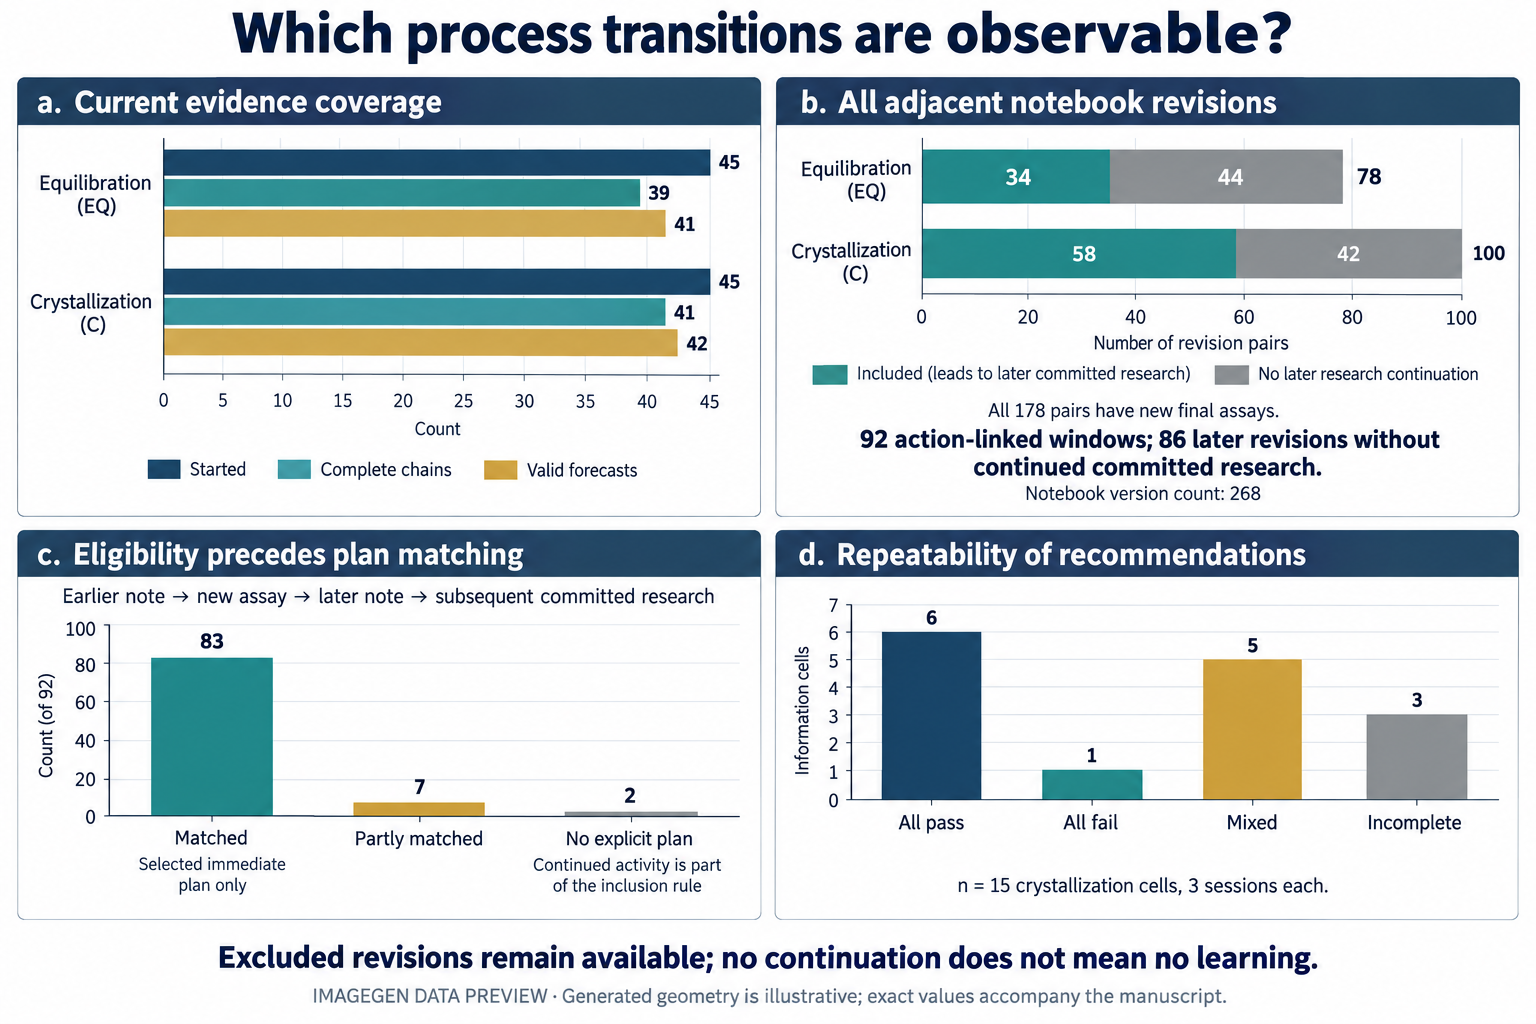
\includegraphics[width=\linewidth,height=.68\textheight,keepaspectratio]{../figures/preview-20261015/extended01.png}}
\caption{扩展数据图 1 \textbar{} 哪些过程转变能够被观察？ImageGen 数据预览。a，当前会话覆盖和有效预测。b，178 对相邻版本均包含新测定，平衡 34/78 对、结晶 58/100 对还具有后续已提交研究行动，合计 92 个入选窗口；另 86 对修订完整保留但不赋予行动关联编码。c，所选即时计划有 83 个匹配、7 个部分匹配、2 个没有明确下一计划。入选先于语义匹配，但以继续行动为条件；计数不代表学习成功，也不涵盖全部提议。d，十五个结晶世界×信息条件单元各三场，六组全达标、一组全未达标、五组混合、三组缺失。生成几何为示意。}
\end{figure}

\clearpage\begin{figure}[H]
\centering
\pandocbounded{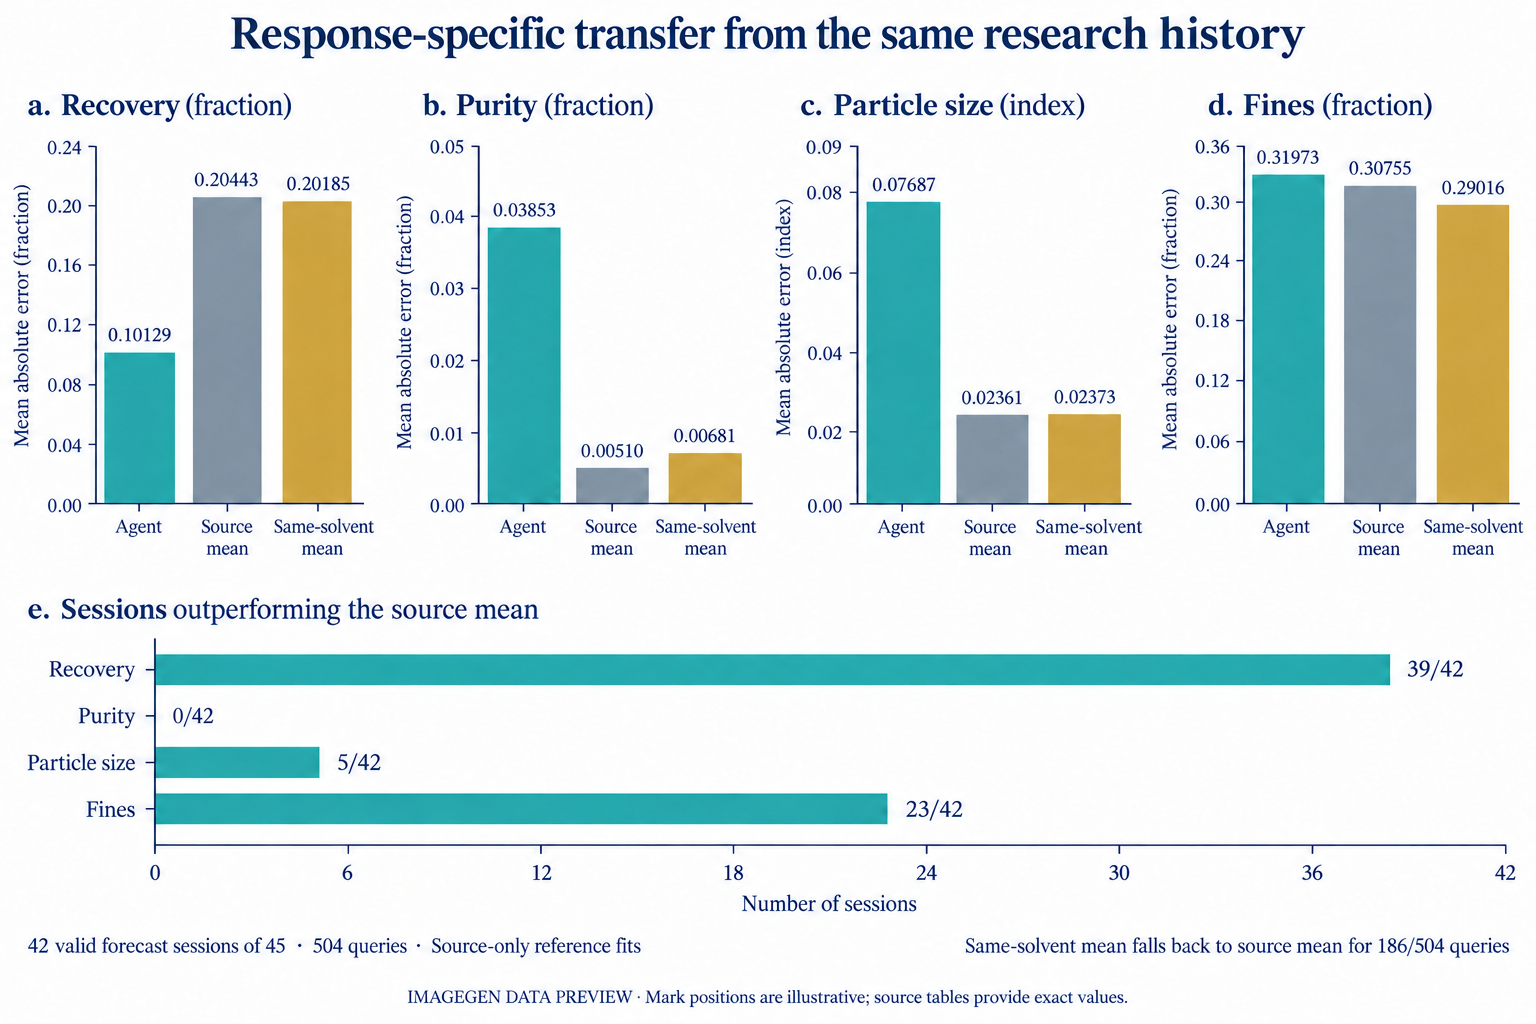
\includegraphics[width=\linewidth,height=.68\textheight,keepaspectratio]{../figures/preview-20261015/extended02.png}}
\caption{扩展数据图 2 \textbar{} 同一研究经历的响应特异性迁移。ImageGen 数据预览。a--d，比较研究者预测与两种仅用源观测拟合的参照，分别展示回收率、纯度、粒径指数和细粉，保留各响应自身尺度。粒径为无量纲指数 min(d50/250 微米, 1)。e，研究者胜过总体源均值的会话数依次为 39/42、0/42、5/42、23/42。修正版结晶 42 份有效预测共含 504 道题；同溶剂参照在 186/504 题回退至总体均值，未匹配热史或数量。两种参照均未使用封存真值拟合。图形位置为示意，五世界等权误差详见补充表。}
\end{figure}

\clearpage\begin{figure}[H]
\centering
\pandocbounded{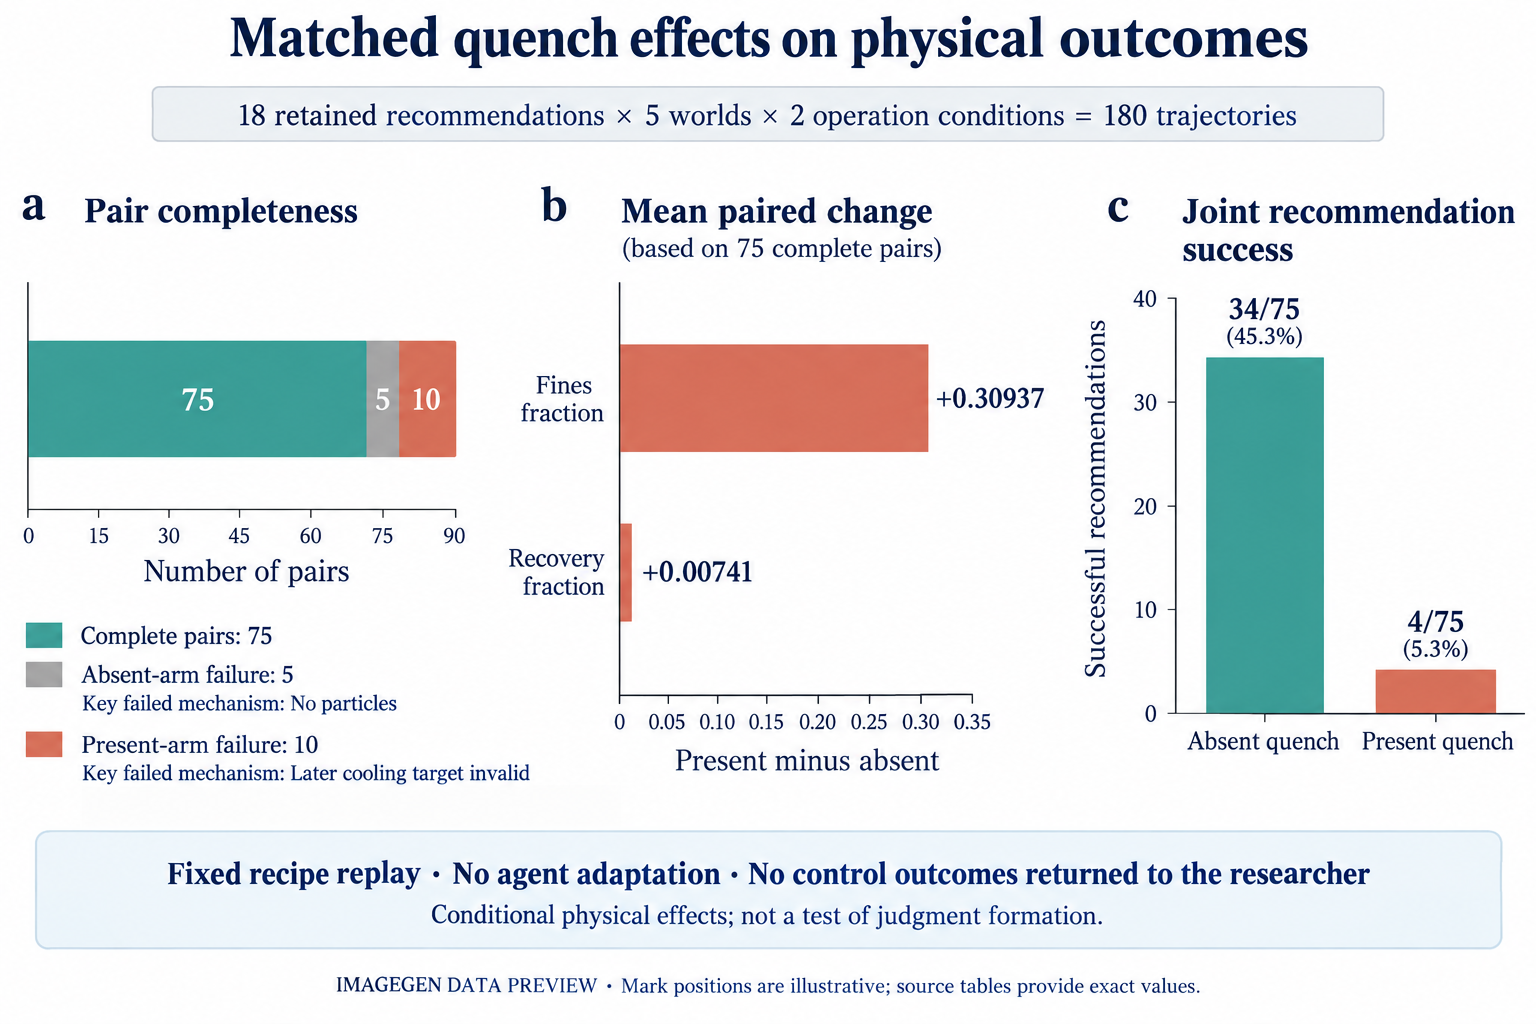
\includegraphics[width=\linewidth,height=.68\textheight,keepaspectratio]{../figures/preview-20261015/extended03.png}}
\caption{扩展数据图 3 \textbar{} 匹配淬灭对物理结果的影响。ImageGen 数据预览。十八份历史推荐在五世界分别有/无淬灭重放，共九十对、一百八十条轨迹。a，七十五对获得双方终测；无淬灭分支五次无颗粒，有淬灭分支十次使后续固定冷却目标无效。b，完整对的细粉平均变化为 +0.30937，回收变化为 +0.00741。c，联合达标从无淬灭 34/75 变为有淬灭 4/75。该结果是初始投料回收定义下的条件性物理作用；研究者未调整操作，也未获得对照结果，因此不能据此识别判断形成原因。图形位置为示意，失败配对全部保留。}
\end{figure}

\end{document}
